% !TEX program = xelatex
% 模版作者： Milvoid，https://shuiyuan.sjtu.edu.cn/t/topic/471743/，https://github.com/Milvoid/CheatingSheetTemplate
% Cheating Paper 作者：dcldyhb
% Built with codex
\RequirePackage{fix-cm}
\documentclass[a4paper]{article}

\usepackage{iftex}
\ifXeTeX
\else
  \errmessage{CheatingSheet.tex must be compiled with XeLaTeX}
\fi

\usepackage[
  a4paper,
  left=0.05cm,
  right=0.05cm,
  top=0.05cm,
  bottom=0.05cm,
  noheadfoot
]{geometry}
\usepackage{fontspec}
\usepackage{xeCJK}
\usepackage{xcolor}
\usepackage{graphicx}
\usepackage{multicol}
\usepackage{titlesec}
\usepackage{enumitem}
\usepackage{amsmath}
\usepackage{amssymb}
\usepackage{mathtools}
\usepackage{array}
\usepackage{booktabs}
\usepackage{tabularx}
\usepackage{tikz}
\usetikzlibrary{decorations.pathreplacing}
\usepackage[colorlinks=true, linkcolor=blue, urlcolor=blue]{hyperref}
\pdfstringdefDisableCommands{%
  \def\quad{ }%
}

% Page and column specification.
\newlength{\CheatColumnWidth}
\newlength{\CheatColumnSep}
\newlength{\CheatTextWidth}
\setlength{\CheatColumnWidth}{5.07cm}
\setlength{\CheatColumnSep}{0.2cm}
\setlength{\CheatTextWidth}{\dimexpr 4\CheatColumnWidth + 3\CheatColumnSep\relax}
\setlength{\textwidth}{\CheatTextWidth}
\setlength{\columnsep}{\CheatColumnSep}
\setlength{\columnseprule}{0pt}
\setlength{\parindent}{0pt}
\setlength{\parskip}{0pt}
\setlength{\topskip}{0pt}
\setlength{\partopsep}{0pt}
\pagestyle{empty}

% Fonts:
% English: SF Compact Text. The bundled files in fonts/ are static Regular,
% Bold, Italic, and BoldItalic instances generated from macOS SF Compact with
% opsz=19. Loading /System/Library/Fonts/SFCompact.ttf directly in XeLaTeX uses
% that variable font's default Black instance, which makes Regular text too bold.
\defaultfontfeatures{Ligatures=TeX}
\newcommand{\CheatFontPath}{fonts/}
\IfFileExists{fonts/SFCompactText-Regular.ttf}{}
  {\renewcommand{\CheatFontPath}{../CheatingSheetTemplate/fonts/}}
\setmainfont{SFCompactText-Regular.ttf}[
  Path=\CheatFontPath,
  BoldFont=SFCompactText-Bold.ttf,
  ItalicFont=SFCompactText-Italic.ttf,
  BoldItalicFont=SFCompactText-BoldItalic.ttf
]
\setsansfont{SFCompactText-Regular.ttf}[
  Path=\CheatFontPath,
  BoldFont=SFCompactText-Bold.ttf,
  ItalicFont=SFCompactText-Italic.ttf,
  BoldItalicFont=SFCompactText-BoldItalic.ttf
]
\setmonofont{SFCompactText-Regular.ttf}[
  Path=\CheatFontPath,
  BoldFont=SFCompactText-Bold.ttf,
  ItalicFont=SFCompactText-Italic.ttf,
  BoldItalicFont=SFCompactText-BoldItalic.ttf
]
% Chinese: PingFang SC, i.e. 苹方-简.
\setCJKmainfont{PingFangSC-Regular.ttf}[
  Path=\CheatFontPath,
  BoldFont=PingFangSC-SemiBold.ttf,
  ItalicFont=PingFangSC-Regular.ttf
]
\setCJKsansfont{PingFangSC-Regular.ttf}[
  Path=\CheatFontPath,
  BoldFont=PingFangSC-SemiBold.ttf,
  ItalicFont=PingFangSC-Regular.ttf
]
\setCJKmonofont{PingFangSC-Regular.ttf}[
  Path=\CheatFontPath,
  BoldFont=PingFangSC-SemiBold.ttf,
  ItalicFont=PingFangSC-Regular.ttf
]
\newfontfamily\CheatLatinSemiBold{SFCompactText-SemiBold.ttf}[
  Path=\CheatFontPath
]
\newfontfamily\CheatLatinSemiBlack{SFCompactText-SemiBlack.ttf}[
  Path=\CheatFontPath
]
\newCJKfontfamily\CheatCJKSemiBold{PingFangSC-SemiBold.ttf}[
  Path=\CheatFontPath
]
\newCJKfontfamily\CheatCJKSemiBlack{PingFangSC-SemiBlack.ttf}[
  Path=\CheatFontPath
]
\xeCJKsetup{
  CJKmath=true,
  CheckSingle=true,
  PunctStyle=kaiming
}

% Typography specification.
\definecolor{CheatTitleRed}{HTML}{a61f38}
\definecolor{CheatAccentBlue}{HTML}{0076BA}
\definecolor{CheatDividerGray}{HTML}{808080}
\makeatletter
\renewcommand\normalsize{%
  \@setfontsize\normalsize{5pt}{6pt}%
  \abovedisplayskip 1pt plus 0.5pt minus 0.5pt%
  \belowdisplayskip 1pt plus 0.5pt minus 0.5pt%
  \abovedisplayshortskip 0.5pt plus 0.5pt%
  \belowdisplayshortskip 0.5pt plus 0.5pt%
}
\makeatother
\normalsize
\DeclareMathSizes{5}{5}{4}{3}
% Compact math spacing for 5 pt cheat-sheet formulas. TeX defaults
% (3/4/5mu) look too loose at this size, especially around +, =, and <.
\thinmuskip=1mu
\medmuskip=1.4mu plus 0.3mu minus 0.5mu
\thickmuskip=1.8mu plus 0.4mu minus 0.6mu

\titleformat{\section}
  {\color{CheatTitleRed}\fontsize{7pt}{7.5pt}\selectfont}
  {}{0pt}{}
\titleformat{\subsection}
  {\color{CheatTitleRed}\fontsize{6pt}{6.5pt}\selectfont\CheatLatinSemiBold\CheatCJKSemiBold}
  {}{0pt}{}
\titlespacing*{\section}{0pt}{1.2pt}{0.6pt}
\titlespacing*{\subsection}{0pt}{0.9pt}{0.4pt}
\setcounter{secnumdepth}{0}

\setlist[itemize]{
  leftmargin=0.85em,
  label={-},
  labelsep=0.25em,
  itemsep=0pt,
  topsep=0pt,
  parsep=0pt,
  partopsep=0pt
}
\setlist[enumerate]{
  leftmargin=1.1em,
  labelsep=0.25em,
  itemsep=0pt,
  topsep=0pt,
  parsep=0pt,
  partopsep=0pt
}
\renewcommand{\arraystretch}{0.95}
\setlength{\tabcolsep}{1.5pt}
\allowdisplaybreaks
\raggedright
\emergencystretch=0.8em

\newenvironment{cheatsheet}
  {\begin{multicols*}{4}\raggedcolumns\normalsize}
  {\end{multicols*}}

\newcommand{\term}[1]{\textbf{#1}}
\newcommand{\accenttext}[1]{{\color{CheatAccentBlue}#1}}
\newcommand{\pointtitle}[1]{{\color{CheatAccentBlue}\CheatLatinSemiBlack\CheatCJKSemiBlack #1}}
\newcommand{\pt}[1]{\pointtitle{#1}}
\newcommand{\paragraphtitle}[1]{\pointtitle{#1}}
\newcommand{\bullettitle}[1]{\pointtitle{#1}}
\newcommand{\m}[1]{\(#1\)}
\newcommand{\tightmath}[1]{\m{#1}}
\newcommand{\divider}{%
  \par\vspace{1pt}%
  {\color{CheatDividerGray}\hrule height 0.5pt width \linewidth}%
  \vspace{1pt}%
}

\newcommand{\tdo}[1]{{\color{CheatTitleRed}\CheatLatinSemiBlack\CheatCJKSemiBlack #1}}

\begin{document}
\begin{cheatsheet}
  \section{第一章\quad 绪论与基本概念}
\pt{工程热力学定义}：工程热力学是一门研究“热能有效利用”以及“热能和其他形式能量转换规律”的科学。
\pt{核心关注点}：热能如何转化为机械能，机械能如何服务于发电、推进、制冷、供暖等工程装置。
\pt{能源分类}：一次能源是天然存在、未经加工或转换的能源，如太阳能、天然气、石油、煤、水力、风能、地热、核能等\par
\noindent
\begin{minipage}[t]{0.62\linewidth}
  \vspace{0pt}
  \pt{热能动力装置}：从燃料燃烧或其他热源中获得热能，并利用热能得到动力的整套设备，包括燃气动力装置和蒸汽动力装置。
  
  内燃机、燃气轮机、喷气发动机等都属于典型热能动力装置。
\end{minipage}
\hfill
\begin{minipage}[t]{0.34\linewidth}
  \vspace{0pt}
  \centering
  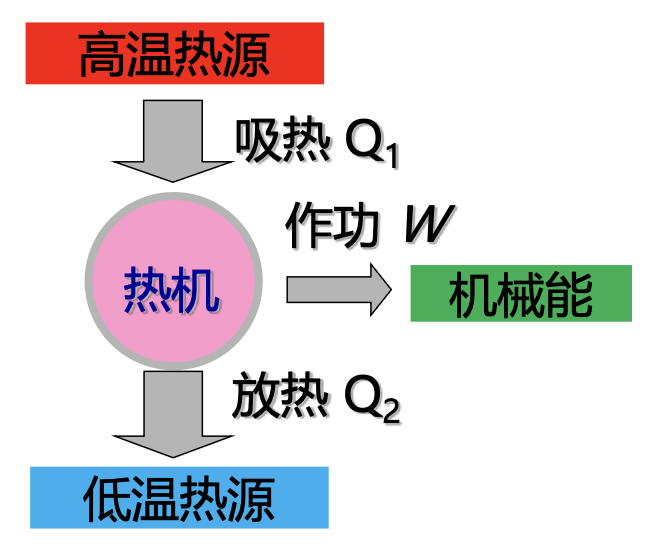
\includegraphics[width=.8\linewidth]{figures/1热机工作过程示意图.png}
  
  {热机过程}
\end{minipage}

\pt{工质}是实现热能和机械能相互转化的媒介物质,应具有\pt{适宜的膨胀性}、\pt{优良的流动性}、\pt{较大的热容量}、\pt{可靠的稳定性和安全性}、\pt{环境友好性}，并且\pt{价廉、容易大量获得}。\pt{热源}是工质从中吸取或向之排出热能的物质系统

\divider
\pt{热力系统}是\pt{人为分割}出来，作为热力学研究对象的有限物质系统
\pt{外界}是与体系发生质量、能量交换的物系
\pt{边界}是系统与外界的分界线
\pt{热力学系统的分类}
\begin{itemize}
  \item 按组元数分：
        \pt{单元系}：由单一纯物质组成，仅含有一种化学成分（\pt{分子种类相同}）；
        \pt{多元系}：系统由两种或以上组分组成，可以是混合物或溶液。
  \item 按相数分：
        \pt{单相系}：系统内所有物质处于\pt{同一相态}，宏观上没有界面分隔，可以是单元系也可以是多元系；
        \pt{复相系}：复相系内同时存在\pt{两种或以上相态}，相之间有\pt{明确界面}，各相性质不同。
  \item 按系统内部状态分：
        \pt{均匀系}：内部各部分物理性质和化学组成完全相同，温度、压力、密度、浓度等处处一致；
        \pt{非均匀系}：存在宏观界面，不同部分性质或组成有明显差异
  \item 按系统与外界质量交换分
        \pt{闭口系}：控制\pt{质量} CM，没有质量越过边界；
        \pt{开口系}：控制\pt{体积} CV，允许质量越过边界。
  \item 按能量交换分
        \pt{绝热系}：与外界没有热量交换，但是可以有功交换或者质量交换；
        \pt{孤立系 ISO}：与外界没有任何形式的质量或者能量交换。
  \item 简单可压缩系：由可压缩物质组成，如水蒸气、空气、燃气等；无化学反应；与外界交换容积变化功，是本课程中讨论的绝大部分系统。
\end{itemize}
这些分类不能简单等同：单元系未必均匀，例如气液平衡分离状态；复相系也未必宏观不均匀，例如湿蒸汽

\divider
\pt{热力学状态}是工质所呈现的宏观物理状况。\pt{状态参数}是描述工质状态的\pt{宏观}物理量；是大量分子运动的宏观平均效果，只有平衡态才有明确状态参数；是状态的单值函数，物理上与\pt{过程无关}，数学上\pt{其微量是全微分}，并且闭合积分为 $0$，$\oint\,\mathrm{x} = 0$。分为\pt{广延量}和\pt{强度量}两类，前者与系统质量成正比，后者与系统质量无关。

系统两个状态相同的充要条件是所有状态参数一一对应相等；对简单可压缩系，两个独立状态参数对应相等即可确定状态相同。

温度是物体冷热程度的标志，测温基础是\pt{热力学第零定律}，即若两个热力学系统均与第三个系统处于热平衡状态，此两个系统也必互相处于热平衡

$$
  \{t\}_{^\circ C}=\{t\}_K - 273.15
$$

\pt{压力}是单位面积上施加的垂直作用力，包括绝对压力 $p$、表压力 $p_\mathrm{e}$ 或 $p_\mathrm{g}$、真空度 $p_\mathrm{v}$、当地大气压 $p_\mathrm{b}$。当系统压力高于大气压：$p = p_\mathrm{b} + p_\mathrm{e}$。当系统压力低于大气压：$p = p_\mathrm{b} - p_\mathrm{v}$。

比体积是单位质量工质的体积：$v = \frac{V}{M}$，单位 $m^3/kg$，密度是单位体积工质的质量：$\rho = \frac{M}{V}$，单位 $kg/m^3$，两者互为倒数：$v = \frac{1}{\rho}$。

\divider
\vspace{0pt}
\pt{热力学过程}是系统状态发生变化的过程，分为\pt{平衡过程}和\pt{非平衡过程}两类。前者系统始终处于热力学平衡态，后者系统至少存在一个状态参数不均匀分布或者存在不可逆现象。

\pt{热力学循环}是系统经历一系列状态变化后回到初始状态的过程。


\pt{热力学能} $U$ 是状态参数，单位为 $J$，一般情况下可写成 $U=U(T,v)$，微分形式为 $\mathrm{d}U=\left(\frac{\partial U}{\partial T}\right)_V\mathrm{d}T+\left(\frac{\partial U}{\partial V}\right)_T\mathrm{d}V=c_V\mathrm{d}T+\left[T\left(\frac{\partial p}{\partial T}\right)_V-p\right]\mathrm{d}V$

\begin{center}
  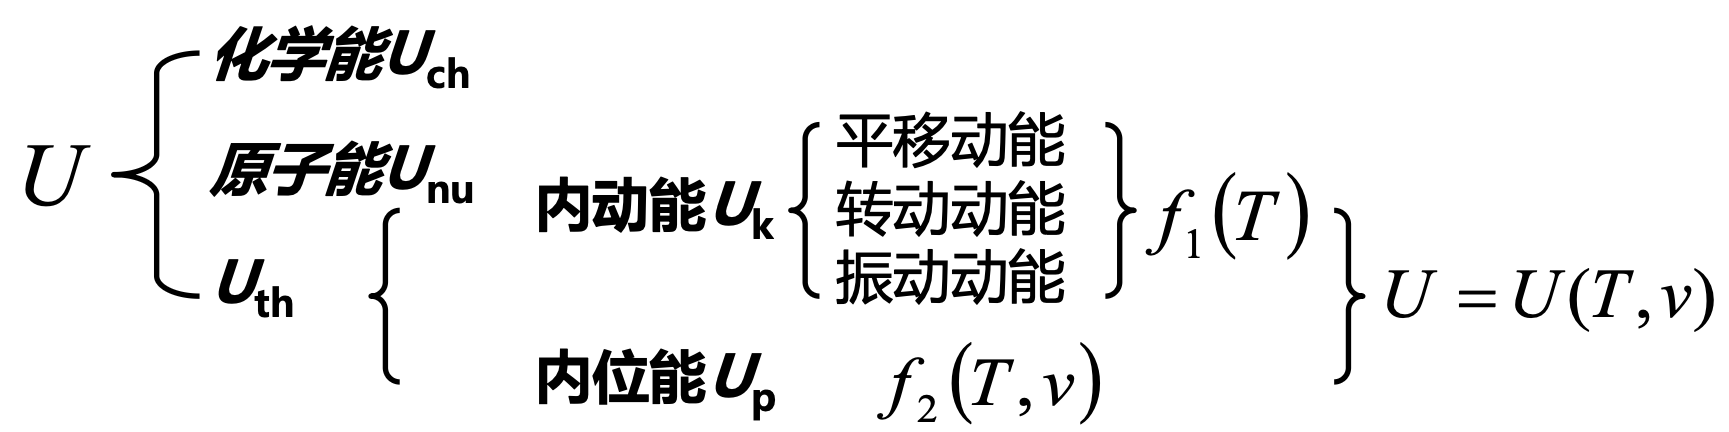
\includegraphics[width=\linewidth]{figures/1热力学能组成.png}
  
  {热力学能的组成}
\end{center}

\pt{总（储存）能}包括热力学能、宏观动能和宏观位能 $E=U+E_k+E_p$

\divider
\pt{推动功}是系统引进或排除工质传递的能量，系统引进或排除工质时，由压力作用产生的功 $W = pV$ \newline
\pt{流动功}是系统维持工质流动所需要的功，常表示为 $pv$，体现单位质量工质的流动功
\pt{焓}为 $H=U+PV$，$\mathrm{d}H=c_p\ \mathrm{d}T+\left[v-T\left(\frac{\partial V}{\partial T}\right)_p\right]\ \mathrm{d}p$\newline
\pt{平衡状态}是热力系统在不受外界影响条件下，状态参数不随时间改变的状态。系统达到平衡的充要条件是系统同时达到\pt{热平衡}和\pt{力平衡}
\pt{热平衡}为无外界作用下热力系统各部分之间没有热量的传递，系统内部、系统与外界处处\pt{温度相等}；
\pt{力平衡}为无外界作用下，系统各部分之间没有相对位移，系统内部、系统与外界处处\pt{压力相等}。
\pt{状态方程}为 $f(p,V,T)=0$

\divider
\pt{准静态过程}为偏离平衡态无穷小，随时恢复平衡的状态变化过程，可在状态参数图上用连续实线表示。进行条件为坏平衡的\pt{势差无穷小}；过程进行无限\pt{缓慢}；工质具有\pt{恢复平衡}的能力。\newline
\pt{可逆过程}为系统可\pt{经原途径返回原来状态}而\pt{在外界不留下任何变化}的过程。可逆过程为\pt{无耗散效应}的\pt{准静态过程}。

\divider

  \section{第二章\quad 热力学第一定律}

热是能的一种，机械能和热能之间相互转换的时候比值是一定的。实质是能量守恒与转换定律在热能与机械能相互转换中的应用

\pt{热力学第一定律基本能量方程}：

$$
    \left(\delta Q + \sum \delta m_i e_i\right) - \left(\delta W_\text{total}+\sum \delta m_je_j\right) = \mathrm{d}E
$$

\pt{闭口系基本能量方程}（热力学第一定律第一解析式）：

$$
    \left\{
    \begin{aligned}
         & Q=\Delta U+W                      \\
         & \delta Q = \mathrm{d}U + \delta W
    \end{aligned}
    \right.
$$

\pt{稳定流动能量方程}:

$$
    \begin{aligned}
        Q=(H_2-H_1) & +q_m\left(\frac{c_{f2}^2}{2}-\frac{c_{f1}^2}{2}\right) \\
                    & +q_mg(z_2-z_1)+W_s
    \end{aligned}
$$

\pt{技术功} $w_t=w_s+\frac{1}{2}\Delta c_f^2+g\Delta z=- \int_{1}^{2} v \, \mathrm{d}p$

\pt{热力学第一定律第二解析式}：$\delta q =\Delta h-v\mathrm{d}p$

\divider
  \section{第三章\quad 气体和蒸汽的性质}
\pt{理想气体}假设分子为不占体积的弹性质点，认为除碰撞外分子间无作用力，是实际气体在\pt{低压高温的抽象}，主要是\pt{低压}

\pt{理想气体状态方程}

$$
    \left\{
    \begin{aligned}
         & pV=mR_{\mathrm{g}}T &  & \text{质量为} m      \\
         & pv=R_{\mathrm{g}}T  &  & 1\,\mathrm{kg} 气体 \\
         & pV=nRT              &  & \text{物质的量为} n
    \end{aligned}
    \right.
$$

$R=8.3145\,\mathrm{J/(mol\cdot K)}$

\divider

\pt{比热容} $\displaystyle c=\lim_{\Delta T\to 0}\frac{q}{\Delta T}=\frac{\delta q}{\mathrm{d}T}$，通常是温度的函数，并且与过程相关

$$
    c=\frac{\partial u}{\partial T}+\left(\frac{\partial u}{\partial v}+p\right)\frac{\mathrm{d}v}{\mathrm{d}T}
$$

\pt{定压比热容} $\displaystyle c_V=\frac{\mathrm{d}h}{\mathrm{d}T}$，
\pt{定容比热容} $\displaystyle c_p=\frac{\mathrm{d}u}{\mathrm{d}T}$，
\pt{迈耶公式} $c_p-c_V=R_\mathrm{g}$，
\pt{比热容比} $\displaystyle \gamma = \frac{c_p}{c_v}$，$\displaystyle c_p=\frac{\gamma R_\mathrm{g}}{\gamma -1}$，$\displaystyle c_V=\frac{R_\mathrm{g}}{\gamma -1}$

\divider

\tdo{水的 $c_p$ 和 $c_v$ 关系，ppt 18 页，待定}

\divider

使用比热容计算热量的途径

\pt{积分计算} $q = \int_{T_1}^{T_2} c\ \mathrm{d}T$，
\pt{平均比热容表} $q=\int_0^{T_2} c\ \mathrm{d}T - \int_0^{T_1} c\ \mathrm{d}T = c_n\vert_0^{T_2}\cdot T_2-c_n\vert_0^{T_1}\cdot T_1$，
\pt{平均比热直线式}：令 $c_n= a + bT$，则 $q = \int_{T_1}^{T_2} (a + bT)\ \mathrm{d}T = a(T_2-T_1)+\frac{b}{2}(T_2^2-T_1^2) = \left(a + \frac{b}{2}(T_1+T_2)\right)(T_2-T_1)$，平均比热容为 $c\vert_{n,t_1}^{t_2}=a+\frac{b}{2}(t_1+t_2)$，
\pt{定值比热容}认为比热容为常数，$q = c(T_2-T_1)$ 根据气体分子运动理论，$C_{V,\mathrm{m}}=\frac{i}{2}R$，$C_{p,\mathrm{m}}=\frac{i+2}{2}R$，$\gamma=\frac{i+2}{i}$，单、双、多原子分子的 $i$ 分别为 $3$ 、$5$ 和 $6$

\divider

\pt{理想气体的热力学能} $\mathrm{d}u = c_V\,\mathrm{d}T$，焓 $\mathrm{d}h = c_p\,\mathrm{d}T$，内能和焓仅是温度的函数，变化量与路径无关。对于\pt{P可逆过程}，理想气体的\pt{熵} $\mathrm{d}s = \frac{\delta q_\mathrm{rev}}{T}=c_V\frac{\mathrm{d}T}{T}+R_{\mathrm{g}}\frac{\mathrm{d}v}{v}$，$\Delta s=\int_{T_1}^{T_2}c_V\frac{\mathrm{d}T}{T}+R_{\mathrm{g}}\ln\frac{v_2}{v_1}=c_V\ln\frac{T_2}{T_1}+R_{\mathrm{g}}\ln\frac{v_2}{v_1}=\int_{T_1}^{T_2}c_p\frac{\mathrm{d}T}{T}-R_{\mathrm{g}}\ln\frac{p_2}{p_1}=c_p\ln\frac{T_2}{T_1}-R_{\mathrm{g}}\ln\frac{p_2}{p_1}$

\divider

\pt{汽化}：液态变为气态的过程；\pt{蒸发}：发生在液体表面的汽化过程；\pt{沸腾}：在液体表面和内部同时进行的剧烈汽化过程；\pt{液化}：气相变为液相的过程。\pt{饱和状态}：气化速度 $=$ 液化速度，宏观上气液两相保持一定的相对数量。饱和温度 $t_s$ 和饱和压力 $p_s$ 一一对应

\pt{饱和液}：处于饱和状态的液体，$t=t_s$；
\pt{干饱和蒸汽}：处于饱和状态的蒸汽，$t=t_s$；
\pt{未饱和液}：温度低于该压力下饱和温度的液体，$t<t_s$；
\pt{过热蒸汽}：温度高于饱和温度的蒸汽，$t>t_s$；
\pt{过热度}：$d=t-t_s$。
使得未饱和液变成饱和液的方法有：保持压力不变升高温度；保持温度不变降低压力。\pt{干度}：湿蒸汽中干饱和蒸汽的质量分数 $x=\frac{m_v}{m_v+m_l}$；
\pt{湿度}：$y=1-x$；
\pt{三相点}：气、液、固三相平衡共存的状态

\divider

水定压加热气化过程：
\pt{预热}：未饱和水升温到饱和水；
\pt{气化}：饱和水变为干饱和蒸汽；
\pt{过热}：干饱和蒸汽继续升温变为过热蒸汽

定压加热过程中的典型状态：
\pt{未饱和水}：$t<t_s$；\pt{饱和水}：$t=t_s$，开始汽化；\pt{湿蒸汽}：$t=t_s$，液、汽共存；\pt{干饱和蒸汽}：$x=1$，汽化结束；\pt{过热蒸汽}：$t>t_s$。

\noindent
\begin{minipage}[t]{0.48\linewidth}
    \vspace{0pt}
    \centering
    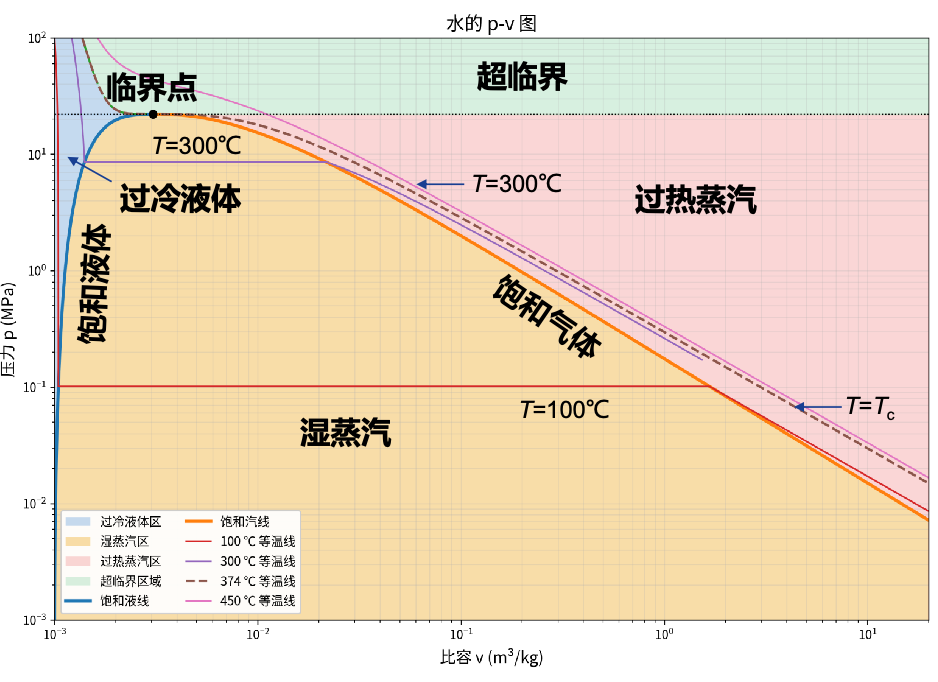
\includegraphics[width=\linewidth]{figures/3水pv图.png}
\end{minipage}
\hfill
\begin{minipage}[t]{0.48\linewidth}
    \vspace{0pt}
    \centering
    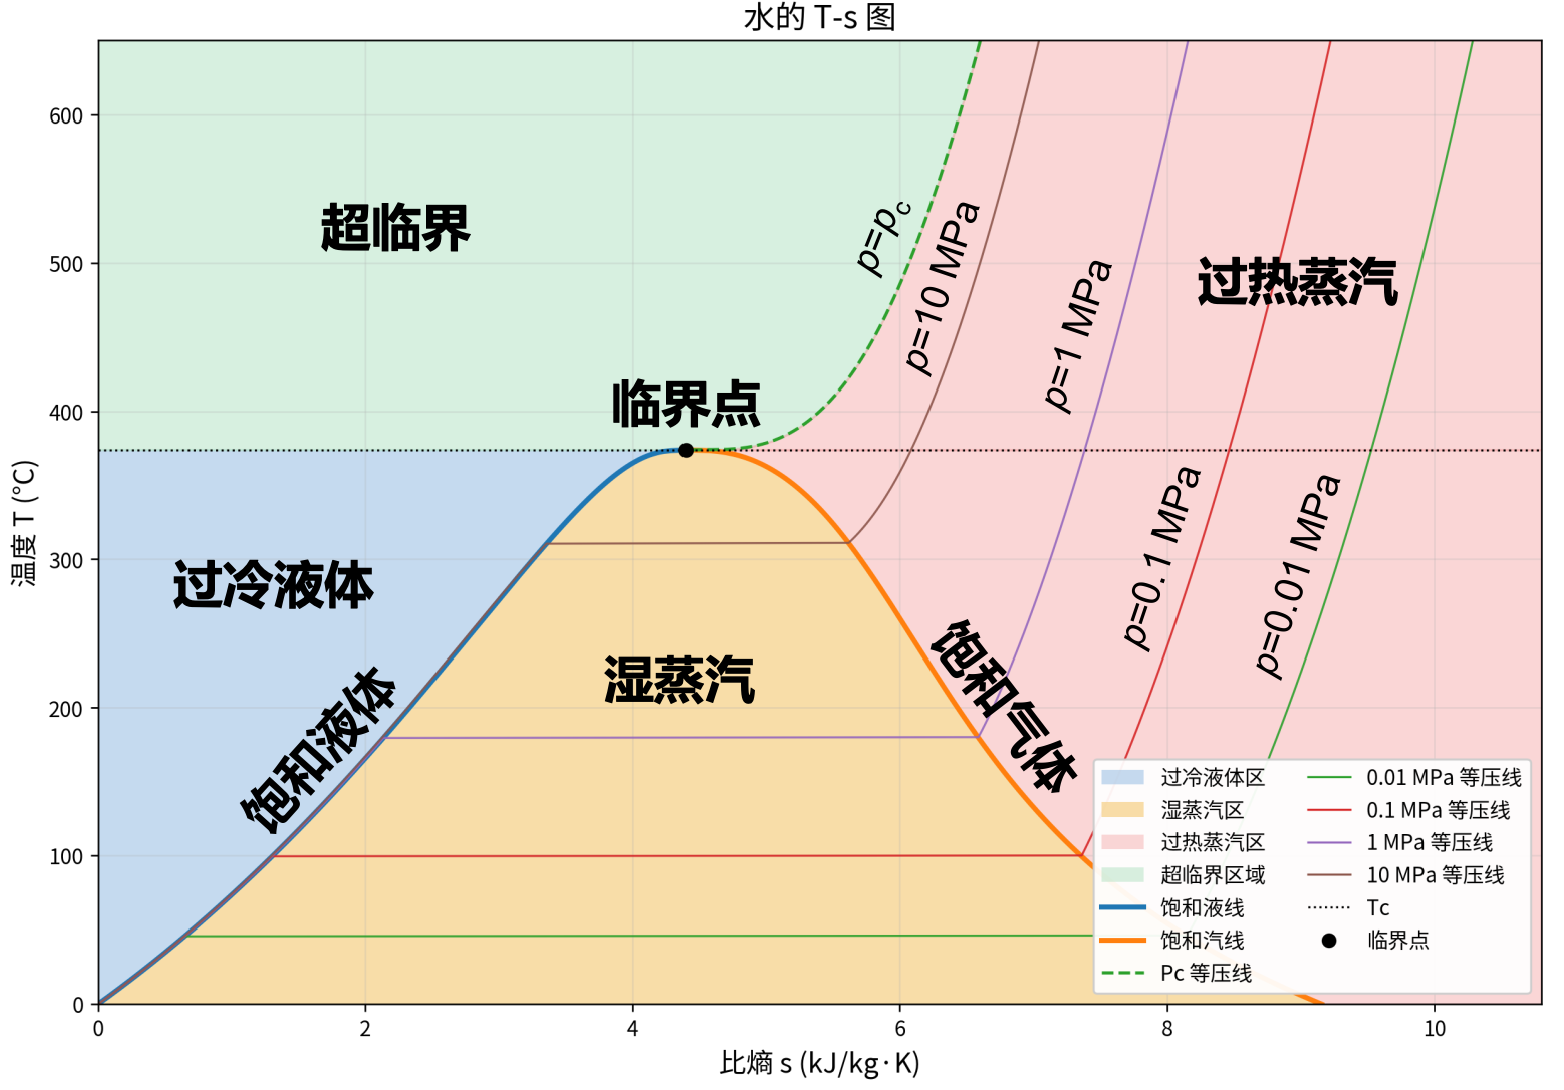
\includegraphics[width=\linewidth]{figures/3水Ts图.png}
\end{minipage}

\divider

动力工程中水蒸气不能用理性想气体性质计算。
规定三相点液态水热力学能和熵为 $0$，$u^\prime_{273.16}=0$，$s^\prime_{273.16}=0$，焓近似为 $0$。

\pt{未饱和水} $(t,p)$ ：查图标或者由专用程序计算得到，压力不太高时近似 $h_t = c_p t$，$s_t=c_p\ln\frac{T}{273.16}$

\pt{饱和水和饱和水蒸气} $p_s$ 或 $t_s$：查表或者程序算

\pt{过热蒸汽} $(p_t)$：查表或者程序算，不能用类似未饱和水的简单近似式

\pt{湿饱和蒸汽} $t_s$ （或 $p_s$）和 $x$：
\pt{比体积} $v_x=xv^{\prime\prime}+(1-x)v^\prime=v^\prime+x(v^{\prime\prime}-v^\prime)$，当 $x$ 较大时 $v_x\approx xv^{\prime\prime}$；
\pt{焓} $h_x=xh^{\prime\prime}+(1-x)h^\prime=h\prime+x(h^{\prime\prime}-h^\prime)$，
$\gamma = h^{\prime\prime}-h^\prime$ 为汽化潜热，可用 $gamma$ 将焓化为 $h_x=h^\prime+x\gamma$，$s_x=xs^{\prime\prime}+(1-x)s^\prime=s^\prime+x(s^{\prime\prime}-s^\prime)$；
\pt{熵}：$s_x=xs^{\prime\prime}+(1-x)s^\prime=s^\prime+x(s^{\prime\prime}-s^\prime)$，饱和相变中 $s^{\prime\prime}-s^\prime=\frac{\gamma}{T_s}$，则 $s_x=s^\prime+x\frac{\gamma}{T_s}$；
\pt{热力学能}：$u_x=h_x-p_sv_x$

\divider
  \section{第四章\quad 理想气体混合物及湿空气}
% 只考 1、2

若各组分气体均处于理想气体状态，则混合气体也可作为理想气体处理。混合气体可等效为某种“假想气体”，其总质量、总物质的量等于各组分之和。

\pt{混合气体状态方程} $pV=mR_{\mathrm{g,eq}}T$;
\pt{平均摩尔质量与折合气体常数关系}：$M_{\mathrm{eq}}R_{\mathrm{g,eq}}=R$；
\pt{物质的量与平均摩尔质量}：$n_{\mathrm{eq}}=\sum_i n_i,n_{\mathrm{eq}}M_{\mathrm{eq}}=\sum_i n_iM_i$ 因此：$M_{\mathrm{eq}}=\sum_i x_iM_i,R_{\mathrm{g,eq}}=\frac{R}{M_{\mathrm{eq}}}$，$R_{\mathrm{g,eq}}=\sum_i w_iR_{\mathrm{g},i},M_{\mathrm{eq}}=\frac{1}{\sum_i \frac{w_i}{M_i}}$

\pt{道尔顿分压定律}：$p=\sum_i p_i$；
\pt{分容积定律}：$V=\sum_i V_i$
\pt{混合气体的质量分数}：$w_i=\frac{m_i}{m},\qquad \sum_i w_i=1$ ；
\pt{混合气体的摩尔分数}：$x_i=\frac{n_i}{n},\qquad \sum_i x_i=1$ ；
\pt{混合气体的体积分数}：$y_i=\frac{V_i}{V},\qquad \sum_i y_i=1$ ；
\pt{混合气体的比热容}：$c_{\mathrm{mix}}=\sum_i w_ic_i$；
\pt{混合气体的热力学能}：$U_{\mathrm{mix}}=\sum_i U_i$；
\pt{混合气体的焓}：$H_{\mathrm{mix}}=\sum_iH_i=\sum_i(U_i+p_iV)=U_{\mathrm{mix}}+pV$；
\pt{混合气体熵}：$S_{\mathrm{mix}}=\sum_iS_i=\sum_i m_is_i$；
无化学反应混合气体过程熵变，按 $1\,\mathrm{kg}$ 混合气体：$\mathrm{d}s_{\mathrm{mix}}=\sum_i w_i\mathrm{d}s_i=\sum_i w_i\left(c_{p,i}\frac{\mathrm{d}T}{T}-R_{\mathrm{g},i}\frac{\mathrm{d}p_i}{p_i}\right)$；
定比热容时：$  \Delta s_{\mathrm{mix}}=\sum_i w_ic_{p,i}\ln\frac{T_2}{T_1}-\sum_i w_iR_{\mathrm{g},i}\ln\frac{p_{i,2}}{p_{i,1}}$；
按 $1\,\mathrm{mol}$ 混合气体：$\mathrm{d}S_{\mathrm{m,mix}}=\sum_i x_iC_{p,\mathrm{m},i}\frac{\mathrm{d}T}{T}-\sum_i x_iR\frac{\mathrm{d}p_i}{p_i}$

\divider

大气由 $\mathrm{N_2}$、$\mathrm{O_2}$、$\mathrm{Ar}$、$\mathrm{CO_2}$、水蒸气及微量气体组成；
若空气中水蒸气为过热状态，$t>t_s(p_{\mathrm{v}})$，则湿空气未饱和；若空气中水蒸气达到饱和，$t=t_s(p_{\mathrm{v}})$，则湿空气饱和；\pt{露点}：湿空气中水蒸气分压力 $p_{\mathrm{v}}$ 所对应的饱和温度称为露点温度

\divider

  \section{第五章\quad 气体和蒸汽的基本热力过程}

% 1到4节

\pt{多变过程}：满足 $p v^n=\mathrm{const.}$ 且 $n=\mathrm{const.}$ 的可逆过程称为多变过程，$n$ 称为\pt{多变指数}。$n=0$：$p=\mathrm{const.}$
为定压过程；$n=1$：$p v=\mathrm{const.}$，对理想气体，表示定温过程；$n=\kappa$：$p v^\kappa=\mathrm{const.}$，表示定熵过程，也就是可逆绝热过程；$n=\pm\infty$：$v=\mathrm{const.}$，定容过程。

{\renewcommand{\arraystretch}{1.18}
\setlength{\tabcolsep}{1.2pt}
\resizebox{\linewidth}{!}{%
    \begin{tabular}{|c|c|c|c|c|c|}
        \hline
         & 定容 $n=\infty$             & 定压 $n=0$ & 定温 $n=1$ & 定熵 $n=\kappa$ & 多变 $n$ \\
        \hline
        特征
         & $v=\mathrm{const.}$
         & $p=\mathrm{const.}$
         & $T=\mathrm{const.}$
         & $s=\mathrm{const.}$
         & $pv^n=\mathrm{const.}$                                                   \\
        \hline
        $T,p,v$ 关系
         &
        $\frac{T_1}{p_1}=\frac{T_2}{p_2}$
         &
        $\frac{T_1}{v_1}=\frac{T_2}{v_2}$
         &
        $p_1v_1=p_2v_2$
         &
        $\begin{gathered}
                 p_1v_1^\kappa=p_2v_2^\kappa\\
                 T_1v_1^{\kappa-1}=T_2v_2^{\kappa-1}\\
                 T_1p_1^{-(\kappa-1)/\kappa}
                 =T_2p_2^{-(\kappa-1)/\kappa}
             \end{gathered}$
         &
        $\begin{gathered}
                 p_1v_1^n=p_2v_2^n\\
                 T_1v_1^{n-1}=T_2v_2^{n-1}\\
                 T_1p_1^{-(n-1)/n}
                 =T_2p_2^{-(n-1)/n}
             \end{gathered}$                                                   \\
        \hline
        $\Delta u$
         & $c_{\mathrm{V}}(T_2-T_1)$
         & $c_{\mathrm{V}}(T_2-T_1)$
         & $0$
         & $c_{\mathrm{V}}(T_2-T_1)$
         & $c_{\mathrm{V}}(T_2-T_1)$                                                \\
        \hline
        $\Delta h$
         & $c_p(T_2-T_1)$
         & $c_p(T_2-T_1)$
         & $0$
         & $c_p(T_2-T_1)$
         & $c_p(T_2-T_1)$                                                           \\
        \hline
        $\Delta s$
         &
        $c_{\mathrm{V}}\ln\frac{T_2}{T_1}$
         &
        $c_p\ln\frac{T_2}{T_1}$
         &
        $\begin{gathered}
                 \frac{q}{T}\\
                 R_{\mathrm{g}}\ln\frac{v_2}{v_1}\\
                 R_{\mathrm{g}}\ln\frac{p_1}{p_2}
             \end{gathered}$
         &
        $0$
         &
        $\begin{gathered}
                 c_{\mathrm{V}}\ln\frac{T_2}{T_1}
                 +R_{\mathrm{g}}\ln\frac{v_2}{v_1}\\
                 c_p\ln\frac{T_2}{T_1}
                 -R_{\mathrm{g}}\ln\frac{p_2}{p_1}\\
                 c_{\mathrm{V}}\ln\frac{p_2}{p_1}
                 +c_p\ln\frac{v_2}{v_1}
             \end{gathered}$                               \\
        \hline
        比热容 $c$
         &
        $c_{\mathrm{V}}=\frac{R_{\mathrm{g}}}{\kappa-1}$
         &
        $c_p=\frac{\kappa R_{\mathrm{g}}}{\kappa-1}$
         &
        $\infty$
         &
        $0$
         &
        $c_n=\frac{n-\kappa}{n-1}c_{\mathrm{V}}$                                    \\
        \hline
        过程功 $w$
         &
        $0$
         &
        $\begin{gathered}
                 p(v_2-v_1)\\
                 R_{\mathrm{g}}(T_2-T_1)
             \end{gathered}$
         &
        $\begin{gathered}
                 R_{\mathrm{g}}T\ln\frac{v_2}{v_1}\\
                 R_{\mathrm{g}}T\ln\frac{p_1}{p_2}
             \end{gathered}$
         &
        $\begin{gathered}
                 -\Delta u\\
                 \frac{R_{\mathrm{g}}}{\kappa-1}(T_1-T_2)\\
                 \frac{R_{\mathrm{g}}T_1}{\kappa-1}
                 \left[1-\left(\frac{p_2}{p_1}\right)^{(\kappa-1)/\kappa}\right]
             \end{gathered}$
         &
        $\begin{gathered}
                 \frac{R_{\mathrm{g}}}{n-1}(T_1-T_2)\\
                 \frac{R_{\mathrm{g}}T_1}{n-1}
                 \left[1-\left(\frac{p_2}{p_1}\right)^{(n-1)/n}\right]
             \end{gathered}$                          \\
        \hline
        技术功 $w_{\mathrm{t}}$
         &
        $v(p_1-p_2)$
         &
        $0$
         &
        $w_{\mathrm{t}}=w$
         &
        $\begin{gathered}
                 -\Delta h\\
                 \frac{\kappa R_{\mathrm{g}}}{\kappa-1}(T_1-T_2)\\
                 \frac{\kappa R_{\mathrm{g}}T_1}{\kappa-1}
                 \left[1-\left(\frac{p_2}{p_1}\right)^{(\kappa-1)/\kappa}\right]\\
                 w_{\mathrm{t}}=\kappa w
             \end{gathered}$
         &
        $\begin{gathered}
                 \frac{nR_{\mathrm{g}}}{n-1}(T_1-T_2)\\
                 \frac{nR_{\mathrm{g}}T_1}{n-1}
                 \left[1-\left(\frac{p_2}{p_1}\right)^{(n-1)/n}\right]\\
                 w_{\mathrm{t}}=nw
             \end{gathered}$                         \\
        \hline
        过程热量 $q$
         &
        $\Delta u$
         &
        $\Delta h$
         &
        $\begin{gathered}
                 T(s_2-s_1)\\
                 q=w=w_{\mathrm{t}}
             \end{gathered}$
         &
        $0$
         &
        $\frac{n-\kappa}{n-1}c_{\mathrm{V}}(T_2-T_1)$                               \\
        \hline
    \end{tabular}%
}}

\divider

\noindent
\begin{minipage}[t]{0.48\linewidth}
    \vspace{0pt}
    若经历水加热、汽化、过热三个阶段：
    \pt{液体加热量}：$q_l=h_1-h_0$；\pt{汽化潜热}：$\gamma=h_2-h_1$；\pt{过热热量}：$q_{\mathrm{sup}}=h_3-h_2$；\pt{总定压换热量}：$q_p=h_3-h_0$； 汽化潜热随压力升高而减小
\end{minipage}
\hfill
\begin{minipage}[t]{0.48\linewidth}
    \vspace{0pt}
    \centering
    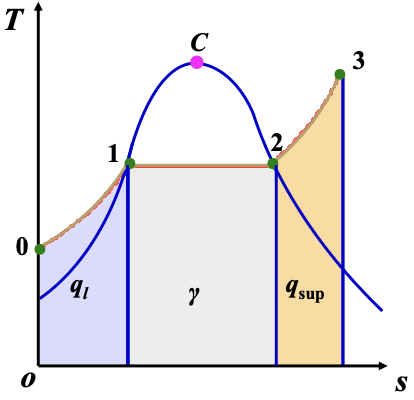
\includegraphics[width=0.8\linewidth]{figures/5水加热的ts图.png}
\end{minipage}

\divider
  \section{第六章\quad 热力学第二定律}

% 1到9

\pt{热力学第二定律的两种表述}：
\pt{克劳修斯表述}：热量不可能自发地、不花代价地从低温物体传向高温物体。
\pt{开尔文表述}：不可能制造一种循环热机，只从单一热源吸热并把它全部转化为功，而不在外界留下任何影响。

\divider

\pt{卡诺循环}是工作在两个恒温热源之间的可逆循环，由两个\pt{可逆等温过程}和两个\pt{可逆绝热过程}组成。正向卡诺循环过程：绝热压缩、等温吸热、绝热膨胀、等温放热。

卡诺热机效率定义为 $\eta_t=\frac{w_{\mathrm{net}}}{q_1}=1-\frac{q_2}{q_1}=\frac{(T_H-T_L)\Delta s}{T_H\Delta s}=1-\frac{T_L}{T_H}$；逆向卡诺制冷循环的制冷系数 $\varepsilon_c=\frac{q_c}{w_{\mathrm{net}}}=\frac{T_c\Delta s}{(T_0-T_c)\Delta s}=\frac{T_c}{T_0-T_c}$； 逆向卡诺供暖循环的供暖系数：$\varepsilon_c'=\frac{q_1}{w_{\mathrm{net}}}=\frac{T_R\Delta s}{(T_R-T_0)\Delta s}=\frac{T_R}{T_R-T_0}>1$; 概括性卡诺循环通过回热、极限回热等方式，使吸热和放热的平均温度关系等效于卡诺循环，效率仍可写为 $\eta_t=1-\frac{T_L\Delta s_{12}}{T_H\Delta s_{34}}=1-\frac{T_L}{T_H}=\eta_c$；多热源可逆循环中定义平均吸热或放热温度

\pt{卡诺定理 1}：在相同 $T_H$ 和 $T_L$ 之间工作的一切可逆循环，热效率相等，与循环种类和工质无关。\pt{卡诺定理 2}：在相同 $T_H$ 和 $T_L$ 之间工作的一切不可逆循环，热效率小于可逆循环热效率 $q=\int_1^2T\,\mathrm{d}s=T_m(s_2-s_1),T_m=\frac{\int_1^2T\,\mathrm{d}s}{s_2-s_1}$，效率为 $\eta_t=1-\frac{q_2}{q_1}=1-\frac{T_{m,2}}{T_{m,1}}$

\divider

\pt{熵} $s$ 是状态参数；其变化只与初终态有关，与过程路径无关。
对\pt{可逆过程}，熵的定义式为 $\mathrm{d}s=\left(\frac{\delta q}{T}\right)_{\mathrm{rev}}$，对任意可逆循环，克劳修斯积分等式为 $\oint \frac{\delta q}{T_r}=0$。
综合可逆与不可逆循环：$\oint \frac{\delta q}{T_r}\leq 0$。

第二定律的过程表达式为 $s_2-s_1\geq \int_1^2\frac{\delta q}{T_r}$，微分形式为 $\mathrm{d}s\geq \frac{\delta q}{T_r}$

理想气体的玻尔兹曼关系式 $S=k\ln W$

\divider

系统熵变化来源包括热量交换导致的\pt{熵流}、质量交换导致的质熵流，以及不可逆过程导致的熵产闭口系熵方程：$\Delta s=s_{\mathrm{f}}+s_{\mathrm{g}}$。\pt{闭口系熵方程}：$\Delta s=s_{\mathrm{f}}+s_{\mathrm{g}}$ ，$s_{\mathrm{f}}=\int_1^2\frac{\delta q}{T_r}$，$s_{\mathrm{g}}\geq 0$

\divider

\noindent
\begin{minipage}
    [t]{0.48\linewidth}
    \vspace{0pt}
    热源热量的作功能力，即\pt{热量㶲}，为热源放出热量理论上可转化为功的最大部分。对平均放热温度为 $T_{m,H}$ 的热源，热量㶲为 $q_a=\left(1-\frac{T_0}{T_{m,H}}\right)q_1$；热量中不可转化为功的部分为\pt{热量㷻}，$q_{\mathrm{un}}=q_1-q_a=\frac{T_0}{T_{m,H}}q_1=T_0\Delta s_{12}$，$q_a=q_1-T_0\Delta s_{12}$

    冷量指低于环境温度传递的热量，冷量㶲为 $q_a=T_0\Delta s_{12}-q_c$，热量㶲与冷量㶲的计算式相差一个符号；热流与热量㶲同向，冷量与冷量㶲反向
\end{minipage}
\hfill
\begin{minipage}
    [t]{0.48\linewidth}
    \vspace{0pt}
    \centering
    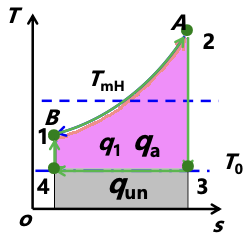
\includegraphics[width=0.8\linewidth]{figures/6热量㶲.png}
    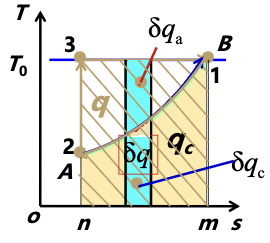
\includegraphics[width=0.8\linewidth]{figures/6冷量㶲.png}
\end{minipage}

\noindent
\begin{minipage}
    [t]{0.48\linewidth}
    \vspace{0pt}
    \pt{闭口系热力学能㶲}：工质因为其状态不同于环境所具备的作功能力，通常是指系统只与环境交换热量可逆过渡到与环境平衡状态作出的最大有用功。
\end{minipage}
\hfill
\begin{minipage}
    [t]{0.48\linewidth}
    \vspace{0pt}
    \centering
    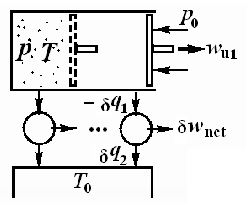
\includegraphics[width=0.8\linewidth]{figures/6热力学能㶲.png}
\end{minipage}

\pt{闭口系热力学㶲}为 $e_{\mathrm{x},U}=u-u_0+p_0(v-v_0)-T_0(s-s_0)$，闭口系从状态 $1$ 到状态 $2$ 的最大有用功：$w_{u,\max,1-2}=e_{\mathrm{x},U,1}-e_{\mathrm{x},U,2}=u_1-u_2-T_0(s_1-s_2)+p_0(v_1-v_2)$

\pt{稳流工质的焓㶲}从状态 $1$ 到状态 $0$ 为 $e_{\mathrm{x},H}=h-h_0-T_0(s-s_0)$，稳流工质从状态 $1$ 到状态 $2$ 可作出的最大有用功为 $w_{u,\max,1-2}=e_{\mathrm{x},H,1}-e_{\mathrm{x},H,2}=h_1-h_2-T_0(s_1-s_2)$，若考虑动能，物流㶲可写为 $e_{\mathrm{x}}=h_1-h_0-T_0(s_1-s_0)+\frac{1}{2}c_{f,1}^2$

机械能可视为\pt{机械㶲}或功㶲，记为 $E_{\mathrm{x},W}$;

热量或冷量的可用能称为\pt{热量㶲}，记为 $E_{\mathrm{x},Q}$，$e_{\mathrm{x},Q}=q_1-T_0(s_2-s_1)$

\pt{㶲损失}与熵产的关系为 $I=T_0S_{\mathrm{g}}=T_0\Delta S_{\mathrm{iso}}$，适用于所有情况、

\pt{闭口系}㶲平衡方程：$E_{\mathrm{x},Q}-W_u - I =E_{\mathrm{x},U_2}-E_{\mathrm{x},U_1}$

\pt{开口系}㶲平衡方程：$Q-Q_0=H_2-H_1+\frac{m}{2}c_{\mathrm{f}2}-\frac{m}{2}c_{\mathrm{f}1}^2+W_\mathrm{s}$

\divider

㶲不守恒：与孤立系熵只增不减相反，孤立系中的\pt{㶲只减不增};\pt{㶲平衡}总表达：流入系统的各种㶲量之和 $-$ 离开系统的各种㶲量之和 $-$ 不可逆过程造成的㶲损失 $=$ 系统㶲变化量，即 $E_{\mathrm{x},Q}-W_u-I=E_{\mathrm{x},U,2}-E_{\mathrm{x},U,1}$。㶲损失即为作功能力损失，均可以以 $T_0S_\mathrm{g}$ 的形式计算

㶲效率为 $\eta_{\mathrm{ex}}=\frac{E_{\mathrm{x},\mathrm{收益}}}{E_{\mathrm{x},\mathrm{代价}}}=\frac{W_s}{E_{\mathrm{x},1}}=\frac{W_s+E_{\mathrm{x},2}}{E_{\mathrm{x},1}}=\frac{W_s}{E_{\mathrm{x},1}-E_{\mathrm{x},2}}$（\pt{后面三项是不同写法，并不是等式}）

\divider

  \section{第七章\quad 气体与蒸汽的流动}

% 1,2,3,5,6，也就是 ppt 上的所有内容

\pt{三维非定常流动连续性方程}：$\frac{\partial\rho}{\partial t}+\frac{\partial(\rho u)}{\partial x}+\frac{\partial(\rho v)}{\partial y}+\frac{\partial(\rho w)}{\partial z}=0$;

\pt{连续性方程}：$\frac{Ac_\mathrm{f}}{\nu}=\text{const.}$;

\pt{微分形式}：$\frac{\mathrm{d}\nu}{\nu}=\frac{\mathrm{d}A}{A}+\frac{\mathrm{d}c_\mathrm{f}}{c_\mathrm{f}}$ 或 $\frac{\mathrm{d}\rho}{\rho}+\frac{\mathrm{d}A}{A}+\frac{\mathrm{d}c_f}{c_f}=0$;

\pt{绝热方程}: $pv^\kappa=\mathrm{const.}$ 微分形式：$\kappa\frac{\mathrm{d}v}{v}+\frac{\mathrm{d}p}{p}=0$；注意，水蒸气中的 $\kappa\ne \frac{c_p}{c_V}$；

\pt{稳定流动能量方程}：$q=\Delta h+\frac{1}{2}\Delta c_f^2+g\Delta z+w_s$， 喷管等问题中常取 $q\approx 0$、$w_s=0$，并忽略 $g\Delta z$，于是：$h+\frac{c_f^2}{2}=\mathrm{const.}$，微分形式为 $\mathrm{d}h+c_f\,\mathrm{d}c_f=0$

\pt{绝热滞止状态}：若流体被绝热、可逆地减速到 $c_f\to 0$，则焓达到最大值：$h_0=h_1+\frac{c_{f1}^2}{2}$， $h_0$ 称为总焓或滞⽌焓

\pt{理想气体、定比热时滞止参数}： $T_0=T_1+\frac{c_{f1}^2}{2c_p},p_0=p_1\left(\frac{T_0}{T_1}\right)^{\frac{\kappa}{\kappa-1}},v_0=\frac{R_gT_0}{p_0}$。若为水蒸气则使用前面两个方程再由水蒸气性质图查到

\pt{拉普拉斯声速方程}：$c=\sqrt{\left(\frac{\partial p}{\partial \rho}\right)_s}=\sqrt{-v^2\left(\frac{\partial p}{\partial v}\right)_s}$。等熵过程中 $c=\sqrt{\kappa pv}=\sqrt{\kappa R_\mathrm{g}T}$。\pt{当地声速}是考虑的某留到某一截面上的声速。\pt{马赫数} $\mathrm{Ma}=\frac{c_f}{c}$

\divider

\pt{气体流速改变的力学条件}：$-\frac{\mathrm{d}p}{p}=\kappa \mathrm{Ma}^2\frac{\mathrm{d}c_f}{c_f}$，可以通过流动的能量方程和热力学第一定律的第二解析式得到，速度升高的能量来源是焓㶲转换为机械能。结合绝热过程方程得到 $\mathrm{Ma}^2\frac{\mathrm{d}c_f}{c_f}=\frac{\mathrm{d}v}{v}$

\pt{几何条件}：$\frac{\mathrm{d}A}{A}=\left(\mathrm{Ma}^2-1\right)\frac{\mathrm{d}c_f}{c_f}$。亚音速加速需要渐缩喷管；超音速加速需要渐扩喷管；音速流动时气体截面收缩至最小，此时的\pt{临界截面（喉部截面）}上的 $p_{\mathrm{cr}},T_{\mathrm{cr}},v_{\mathrm{cr}}$ 分别称为临界压力、临界温度、临界比体积。使得气体从亚音速加速到超音速的喷管为\pt{渐缩渐扩喷管}，称为\pt{拉伐尔喷管}

\pt{扩压管}的目的是使得 $p$ 上升，$c_f$ 下降，$\mathrm{Ma}$ 下降，将动能转换为压力势能

\divider

\pt{流速计算}：$c_{f2}=\sqrt{2(h_0-h_2)}=\sqrt{2(h_1-h_2)+c_{f1}^2}$ 适用于绝热、不做功的任意工质。
\pt{理想气体、定比热容}：$c_f=\sqrt{2c_p(T_0-T_2)}=\sqrt{2\frac{\kappa R_{\mathrm{g}}}{\kappa-1}(T_{0}-T_{2})}$，$T_0$ 为滞止温度, $T_0=T_1+\frac{c_{f1}^2}{2c_p},p_0=p_1\left(\frac{T_0}{T_1}\right)^{\frac{\kappa}{\kappa-1}},v_0=\frac{R_gT_0}{p_0}$ \\
若可逆 $c_f=\sqrt{\frac{2\kappa}{\kappa-1}R_gT_0\left[1-\left(\frac{p_2}{p_0}\right)^{\frac{\kappa-1}{\kappa}}\right]}$

\pt{临界压力比}：$\nu_{\mathrm{cr}}=\frac{p_{\mathrm{cr}}}{p_0}=\left(\frac{2}{\kappa+1}\right)^{\frac{\kappa}{\kappa-1}}$

\pt{背压对流速的影响}

\begin{itemize}
    \item \pt{收缩喷管}：若 $p_b>p_{\mathrm{cr}}$，则 $p_2=p_b$，$c_{f2}<c_2$，$\mathrm{Ma}_2<1$。
    \item \pt{收缩喷管}：若 $p_b\le p_{\mathrm{cr}}$，则 $p_2=p_{\mathrm{cr}}$，$c_{f2}=c_2$，$\mathrm{Ma}_2=1$，发生临界流动。
    \item \pt{缩放喷管}：只讨论 $p_b<p_{\mathrm{cr}}$ 的情况，此时 $p_{\mathrm{thr}}=p_{\mathrm{cr}}$，$c_{f,\mathrm{thr}}=c_{\mathrm{cr}}$，$\mathrm{Ma}_{\mathrm{thr}}=1$，出口可达 $\mathrm{Ma}_2>1$。
\end{itemize}

\pt{流量计算}：$q_m=\frac{A c_f}{v}=\rho A c_f$， 通常收缩喷管按出口截面计算；缩放喷管可按喉部截面或出口截面计算。理想气体、定比热容、绝热时 $q_m=A_2\sqrt{\frac{2\kappa}{\kappa-1}\frac{p_0}{v_0}\left[\left(\frac{p_2}{p_0}\right)^{\frac{2}{\kappa}}-\left(\frac{p_2}{p_0}\right)^{\frac{\kappa+1}{\kappa}}\right]}$

\begin{itemize}
    \item 当 $\frac{p_2}{p_0}=1$ 时，$q_m=0$，$c_{f2}=0$。
    \item 当 $\nu_{\mathrm{cr}}<\frac{p_2}{p_0}<1$ 时，$\frac{p_2}{p_0}\downarrow$，$c_{f2}\uparrow$，$q_m\uparrow$。
    \item 当 $\frac{p_2}{p_0}=\nu_{\mathrm{cr}}$ 时，$p_2=p_{\mathrm{cr}}$，$c_{f2}=c_2$，$q_m=q_{m,\max}$。
    \item 当 $\frac{p_2}{p_0}<\nu_{\mathrm{cr}}$ 时，收缩喷管已堵塞，流量仍为 $q_{m,\max}$。
\end{itemize}

\noindent
\begin{minipage}
    [t]{0.48\linewidth}
    \vspace{0pt}
    \raggedright
    \pt{喷管设计任务}：已知 $p_1$,$v_1$,$T_1$,$c_{f1}$,$p_b$,$P$ 确定喷管形状和几何尺寸。\\
    \pt{外形选择}：先比较 $p_{\mathrm{cr}}$ 与 $p_b$，再决定收缩喷管或缩放喷管。\\
    \pt{几何尺寸}：$A_2=\frac{q_m v_2}{c_{f2}}$，$A_{\mathrm{thr}}=\frac{q_m v_{\mathrm{cr}}}{c_{f,\mathrm{cr}}}$，$l=\frac{d_2-d_{\min}}{2\tan(\varphi/2)}$
\end{minipage}
\hfill
\begin{minipage}
    [t]{0.48\linewidth}
    \vspace{0pt}
    \centering
    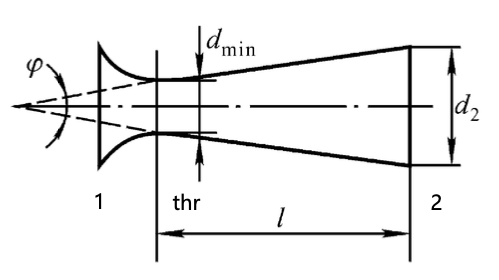
\includegraphics[width=\linewidth]{figures/7喷管设计.png}
\end{minipage}

\divider

摩擦使实际出口速度小于可逆绝热出口速度 $c_{f2}<c_{f2s}$。\\
\pt{喷管速度系数} $\varphi=\frac{c_{f2}}{c_{f2s}}$，一般取 $0.92\sim 0.98$。\\
\pt{能量损失系数}：$\zeta=\frac{c_{f2s}^2-c_{f2}^2}{c_{f2s}^2}=1-\varphi^2$，\\
\pt{喷管效率}：$\eta_N=\frac{c_{f2}^2}{c_{f2s}^2}=\frac{h_0-h_2}{h_0-h_{2s}}=\varphi^2$，$\zeta=1-\eta_N$\\
\pt{摩擦引起的作功能力损失}：$I=\frac{1}{2}\left(c_{f2s}^2-c_{f2}^2\right)$

\divider

\noindent
\begin{minipage}
    [t]{0.48\linewidth}
    \vspace{0pt}
    绝热节流前后焓几乎不变，但是非等焓过程，\\强烈不可逆 $s_2>s_1$，\\做工能力损失 $I=T_0s_g=s_2-s_1$\\
    焦耳-汤姆逊系数：$\mu_J=\left(\frac{\partial T}{\partial p}\right)_h=\frac{T\left(\frac{\partial v}{\partial T}\right)_p-v}{c_p}$
\end{minipage}
\hfill
\begin{minipage}
    [t]{0.48\linewidth}
    \vspace{0pt}
    \centering
    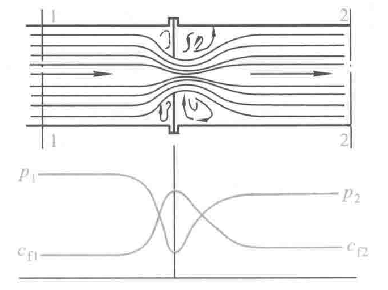
\includegraphics[width=\linewidth]{figures/7绝热节流.png}
\end{minipage}

\begin{itemize}
    \item 若 $T\left(\frac{\partial v}{\partial T}\right)_p-v>0$ 则 $\mu_J>0$，$\mathrm{d}T<0$，节流降温。
    \item 若 $T\left(\frac{\partial v}{\partial T}\right)_p-v<0$ 则 $\mu_J<0$，$\mathrm{d}T>0$，节流升温。
    \item 若 $T\left(\frac{\partial v}{\partial T}\right)_p-v=0$ 则 $\mu_J=0$，$\mathrm{d}T=0$。
\end{itemize}

\pt{回转温度}：节流前后温度保持不变的温度。将气体状态方程带入 $\mu_j$ 式能够得到不同压力下的回转温度，连接得到曲线，根据曲线内外带入点计算 $\mu_J$ 的符号能够判断该点是节流升温还是节流降温。

若为\pt{水蒸气}，则节流后温度稍有下降，前后可取 $h_1=h_1'$，若膨胀到相同压力，节流后的作功能力减少 $(h_1-h_2)-(h_1'-h_2')=h_2'-h_2$，作功能力损失 $I=h_2'-h_2=T_0s_g=T_0(s_1'-s_1)$

\divider
  \section{第八章\quad 压气机的热力过程}

%1、2、3、4 ppt 上全部

\pt{压缩气体用途}：动力机、风动工具、制冷工程、化学工业、潜水作业、医疗、休闲等。

\pt{按压头高低分类}：\pt{通风机}：表压 $<0.01\,\mathrm{MPa}$；\pt{鼓风机}：表压约 $0.1\sim0.3\,\mathrm{MPa}$；\pt{压缩机}：表压 $>0.3\,\mathrm{MPa}$。

\pt{按工作原理分类}：\pt{活塞式}：压头高、流量小、间歇生产；\pt{叶轮式}：压头低、流量大、连续生产。

\pt{压气机特点}：不是动力机，内部进行的是气体压缩与输送过程，不是热力循环。

\noindent
\begin{minipage}
    [t]{0.48\linewidth}
    \vspace{0pt}
    \raggedright
    \pt{单级活塞式基本过程}：
    \begin{itemize}
        \item $0$-$1$：吸气，推动功 $p_1v_1$。
        \item $1$-$2$：压缩，压缩功 $w_{1-2}=-\int_1^2 p\,\mathrm{d}v$。
        \item $2$-$3$：排气，推动功 $p_2v_2$。
    \end{itemize}
\end{minipage}
\hfill
\begin{minipage}
    [t]{0.48\linewidth}
    \vspace{0pt}
    \centering
    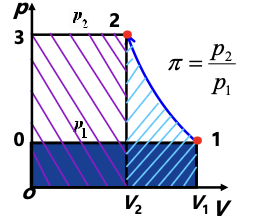
\includegraphics[width=.8\linewidth]{figures/8单级活塞式压气机.png}
\end{minipage}

\pt{压力比}：$\pi=\frac{p_2}{p_1}$

\pt{压气机耗功}：$W_C=\int_1^2V\,\mathrm{d}p=-W_t$，单位质量 $w_C=\int_1^2v\,\mathrm{d}p=-w_t$。生产量常用单位时间生产气体的标准立方米表示，不同于进、排气状态体积。

\noindent
\begin{minipage}
    [t]{0.48\linewidth}
    \vspace{0pt}
    \raggedright
    \pt{理论耗功}：$-w_t=\Delta h-q$，$w_C$ 取决于初终态及过程特征。理想气体：
    \begin{itemize}
        \item \pt{绝热压缩} $q=0$：$w_{C,s}=h_{2s}-h_1=\frac{\kappa}{\kappa-1}R_{\mathrm{g}}T_1\left(\pi^\frac{\kappa-1}{\kappa}-1\right)$。
        \item \pt{等温压缩} $\Delta h=0$：$w_{C,T}=R_{\mathrm{g}}T_1\ln\pi$。
        \item \pt{多变压缩}：$w_{C,n}=\frac{n}{n-1}p_1v_1\left(\pi^\frac{n-1}{n}-1\right)$。
    \end{itemize}

    \pt{压缩过程比较}：$w_{C,s}>w_{C,n}>w_{C,T}$，$T_{2s}>T_{2n}>T_{2T}$，$v_{2s}>v_{2n}>v_{2T}$；\\通常为多变压缩 $1<n<\kappa$，\\$n\uparrow$ 时 $w_{C,n},T_{2n},v_{2n}$ 均增大；\\理想压缩为\pt{等温压缩}。
\end{minipage}
\hfill
\begin{minipage}
    [t]{0.48\linewidth}
    \vspace{0pt}
    \centering
    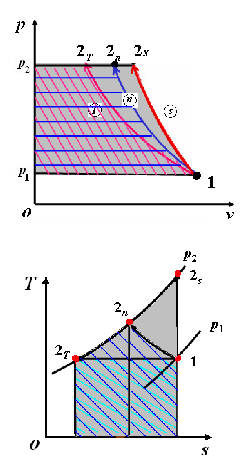
\includegraphics[width=.8\linewidth]{figures/8三种压缩.png}
\end{minipage}

\divider

\noindent
\begin{minipage}
    [t]{0.48\linewidth}
    \vspace{0pt}
    \raggedright
    \pt{余隙容积 $V_c$}：产生于进、排气结构布置、制造装配公差、部件热膨胀等。
    工作过程：
    \begin{itemize}
        \item $1$-$2$ 压缩
        \item $2$-$3$ 排气
        \item $3$-$4$ 余隙气体膨胀
        \item $4$-$1$ 吸气
    \end{itemize}
\end{minipage}
\hfill
\begin{minipage}
    [t]{0.48\linewidth}
    \vspace{0pt}
    \centering
    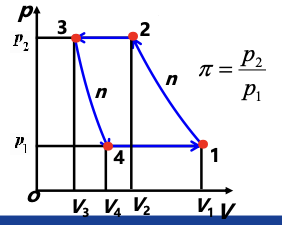
\includegraphics[width=.8\linewidth]{figures/8带余隙容积的压缩.png}
\end{minipage}

\pt{余隙相关容积}：$V_c=V_3$，气缸工作容积 $V_h=V_1-V_3$，\\有效吸气容积 $V_{\mathrm{es}}=V_1-V_4$，余隙容积比 $\sigma=\frac{V_c}{V_h}$。\\\pt{每周期生产量} $m_{\mathrm{pr}}=m_1\frac{V_1-V_4}{V_1}$。

\noindent
\begin{minipage}
    [t]{0.58\linewidth}
    \vspace{0pt}
    \raggedright
    \pt{容积效率}：$\eta_V=\frac{V_{\mathrm{es}}}{V_h}=\frac{V_1-V_4}{V_1-V_3}=1-\frac{V_3}{V_1-V_3}\left(\frac{V_4}{V_3}-1\right)=1-\sigma\left(\pi^{1/n}-1\right)$。
    \begin{itemize}
        \item $V_c,V_h$ 定时：$\pi\uparrow\Rightarrow\eta_V\downarrow,m_p\downarrow$。
        \item $\pi$ 定时：$V_c\uparrow\Rightarrow V_{\mathrm{es}}\downarrow,\eta_V\downarrow,m_p\downarrow$。
    \end{itemize}
\end{minipage}
\hfill
\begin{minipage}
    [t]{0.38\linewidth}
    \vspace{0pt}
    \centering
    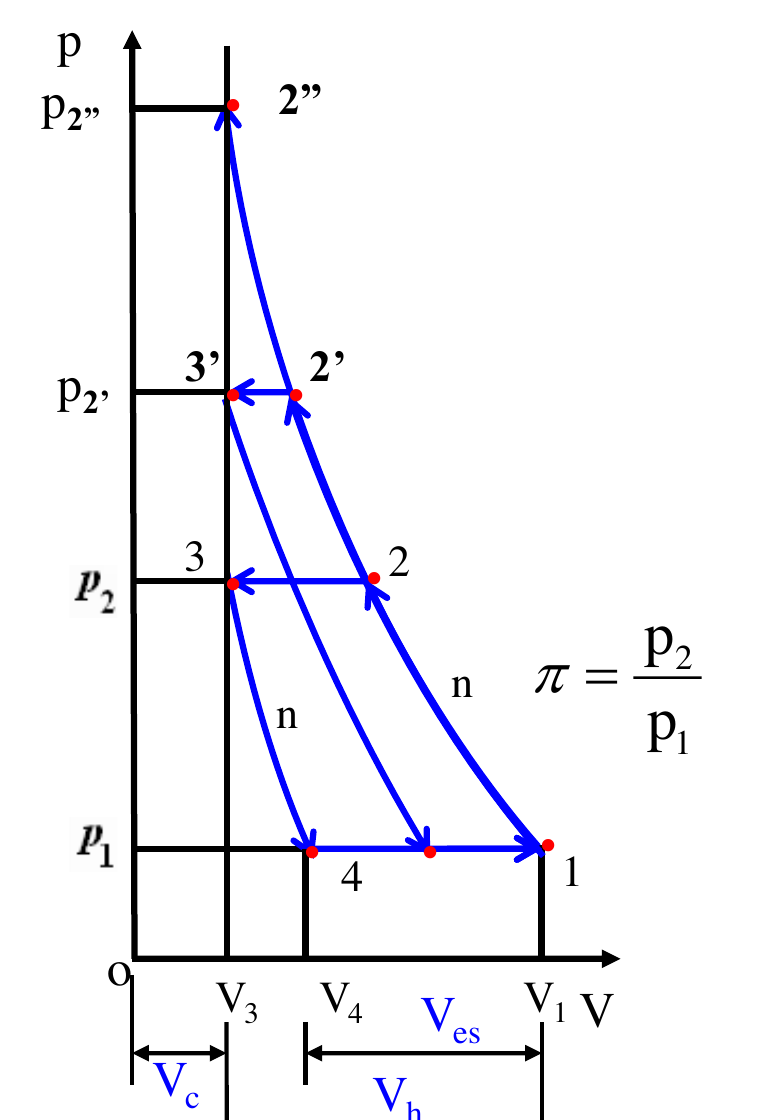
\includegraphics[width=.8\linewidth]{figures/8余隙容积效率影响.png}
\end{minipage}

\pt{余隙对理论耗功}：$W_C=W_{t,1-2}-W_{t,3-4}=\frac{n}{n-1}p_1(V_1-V_4)\left(\pi^{(n-1)/n}-1\right)$；因 $V_{\mathrm{es}}=m_{\mathrm{pr}}v_1$，故 $w_C=\frac{W_C}{m_{\mathrm{pr}}}=\frac{n}{n-1}v_1p_1\left(\pi^{(n-1)/n}-1\right)$。余隙使生产量下降、实际耗功增大，但对生产 $1\,\mathrm{kg}$ 气体的理论耗功无影响，故称有害容积。

\divider


\pt{叶轮式压气机}：包括轴流式、离心式；转速高，连续吸排气，运转平稳，排气量大，无余隙影响，但每级压比不高。因排量大、转速高、难冷却，常按\pt{绝热压缩}分析。

\noindent
\begin{minipage}
    [t]{0.56\linewidth}
    \vspace{0pt}
    \raggedright
    \pt{叶轮式绝热分析}：理论耗功 $w_{C,s}=h_{2s}-h_1$，实际耗功 $w'_C=h_{2'}-h_1$，实际多耗功 $\Delta w_C=h_{2'}-h_{2s}$。绝热内效率
    $\eta_{C,s}=\frac{w_{C,s}}{w'_C}=\frac{h_{2s}-h_1}{h_{2'}-h_1}$；理想气体时 $\eta_{C,s}=\frac{T_{2s}-T_1}{T_{2'}-T_1}$，$T_{2'}=T_1+\frac{T_{2s}-T_1}{\eta_{C,s}}=T_1+\frac{w_{\mathrm{c}}'}{c_\mathrm{p}}$。
\end{minipage}
\hfill
\begin{minipage}
    [t]{0.40\linewidth}
    \vspace{0pt}
    \centering
    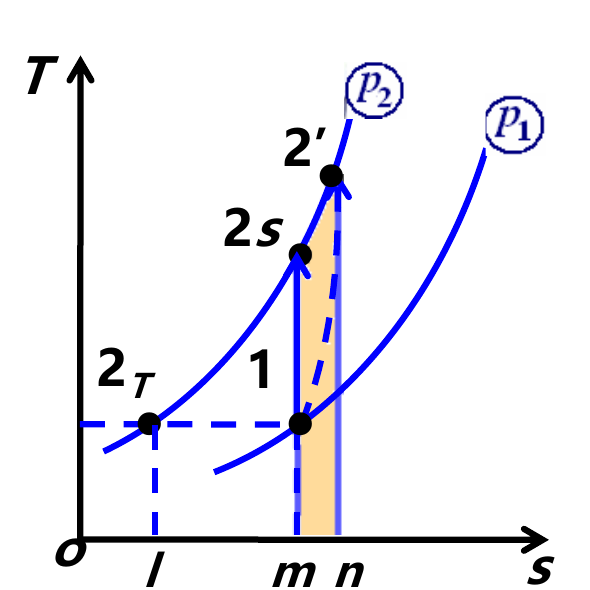
\includegraphics[width=.8\linewidth]{figures/8叶轮式Ts图.png}
\end{minipage}

\newpage

\pt{多级压缩与级间冷却}：高压气体压缩时 $p\uparrow$ 使 $T\uparrow$、$\eta_V\downarrow$，常受 $T_2\leq T_{2,\max}$、$\eta_V\geq\eta_{V,\min}$ 限制，故采用分级压缩、级间冷却。

%\noindent
%\begin{minipage}
%    [t]{0.52\linewidth}
%    \vspace{0pt}
%    \raggedright
%    \pt{多级压缩与级间冷却}：高压气体压缩时 $p\uparrow$ 使 $T\uparrow$、%$\eta_V\downarrow$，常受 $T_2\leq T_{2,\max}$、$\eta_V\geq\eta_%{V,\min}$ 限制，故采用分级压缩、级间冷却。
%\end{minipage}
%\hfill
%\begin{minipage}
%    [t]{0.44\linewidth}
%    \vspace{0pt}
%    \centering
%    \includegraphics[width=.8\linewidth]{figures/8多级压缩装置.png}
%\end{minipage}

\noindent
\begin{minipage}
    [t]{0.56\linewidth}
    \vspace{0pt}
    \raggedright
    \pt{二级压缩耗功}：每生产 $1\,\mathrm{kg}$ 气体，$w_C=w_{C,L}+w_{C,H}$。若中冷后 $T_3=T_1$，令 $a=\frac{n-1}{n}$，$\pi_L=\frac{p_a}{p_1}$，$\pi_H=\frac{p_2}{p_a}$，则 $w_C=\frac{nR_{\mathrm{g}}T_1}{n-1}(\pi_L^a+\pi_H^a-2)$。
\end{minipage}
\hfill
\begin{minipage}
    [t]{0.40\linewidth}
    \vspace{0pt}
    \centering
    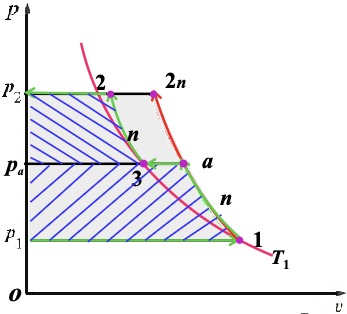
\includegraphics[width=.8\linewidth]{figures/8二级压缩耗功图.png}
\end{minipage}

\pt{最佳中间压力}：令 $\frac{\partial w_C}{\partial p_a}=0$，得 $p_a=\sqrt{p_1p_2}$，即 $\pi_L=\frac{p_a}{p_1}=\frac{p_2}{p_a}=\pi_H$，此时 $w_C=w_{C,\min}$。推广到 $m$ 级：$\pi_1=\pi_2=\cdots=\pi_m=\left(\frac{p_2}{p_1}\right)^{1/m}$。

\pt{等压比分级优点}：各级耗功相等 $w_{C,i}=\frac{n}{n-1}R_{\mathrm{g}}T_1\left(\pi_i^{(n-1)/n}-1\right)$，$w_C=mw_{C,i}$；各缸终温相同 $T_i=T_1\pi_i^{(n-1)/n}$；各级缸散热 $q_i=\frac{n-\kappa}{n-1}c_{\mathrm{V}}\Delta T$、中冷器散热 $q_{\mathrm{中},i}=c_p\Delta T$ 相等；各缸按比例缩小，利于曲轴平衡、润滑可靠和提高整机 $\eta_V$。

\noindent
\begin{minipage}
    [t]{0.56\linewidth}
    \vspace{0pt}
    \raggedright
    \pt{级数影响}：$m\uparrow$ 时趋近等温压缩；但体积庞大、系统复杂、可靠性下降，工程常用 $2$--$4$ 级。\\\pt{定温效率} $\eta_{C,T}=\frac{w_{C,T}}{w_C}$。\\\pt{真空泵}实质也是压气机：出口压力为环境压力，进气压力不断降低。
\end{minipage}
\hfill
\begin{minipage}
    [t]{0.40\linewidth}
    \vspace{0pt}
    \centering
    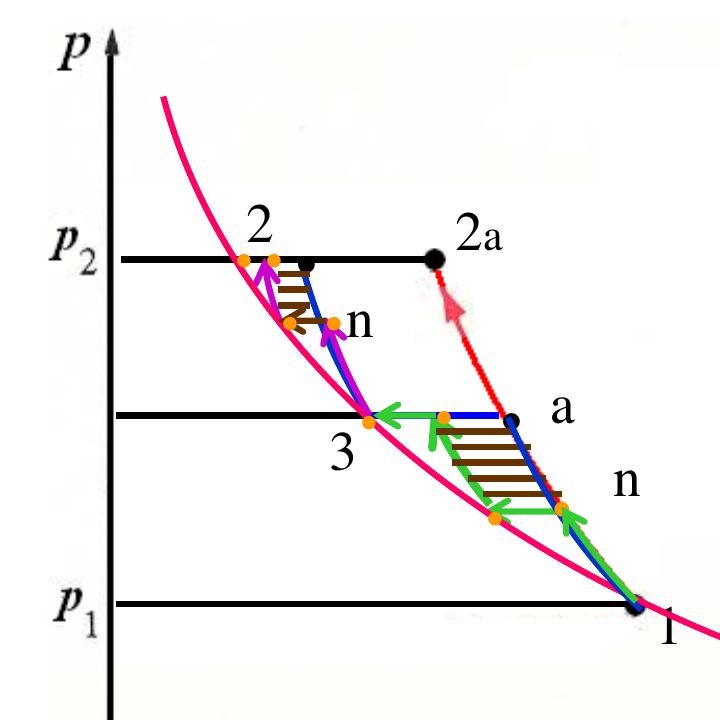
\includegraphics[width=.8\linewidth]{figures/8四级压缩趋等温.png}
\end{minipage}

\divider


  \section{第九章\quad 气体动力循环}

% 1、2、3、4、6、7 ppt 全部

\pt{动力循环分析方法}：将复杂不可逆实际循环抽象为可逆理论循环，先找影响经济性的主要因素，再比较实际循环偏离。第一定律看能量数量，第二定律、熵分析、㶲分析看能量质量与损失。

\pt{活塞式内燃机的分类}

\begin{itemize}
    \item \pt{按燃料}：煤气机、汽油机、柴油机。
    \item \pt{按点火方式}：点燃式、压燃式。
    \item \pt{按冲程}：二冲程、四冲程。
\end{itemize}

\pt{活塞式内燃机循环特点}：实际上是开式循环；燃烧、传热、排气、膨胀、压缩等过程都存在不可逆性；各环节中工质的质量和成分会发生变化。

\pt{空气标准假设}：工质为空气，视为理想气体且定比热；燃烧简化为外部吸热，排气简化为放热；忽略燃料导致的质量、成分变化；压缩和膨胀常取等熵。

\divider

\noindent
\begin{minipage}
    [t]{0.48\linewidth}
    \vspace{0pt}
    \raggedright
    \pt{简化前的混合加热内燃机（柴油机）}：
    \begin{itemize}
        \item $0\to1$：吸气。
        \item $1\to2$：压缩。
        \item $2\to3$：喷油、定容燃烧。
        \item $3\to4$：定压燃烧。
        \item $4\to5$：膨胀作功。
        \item $5\to0$：排气。
    \end{itemize}
\end{minipage}
\hfill
\begin{minipage}
    [t]{0.48\linewidth}
    \vspace{0pt}
    \centering
    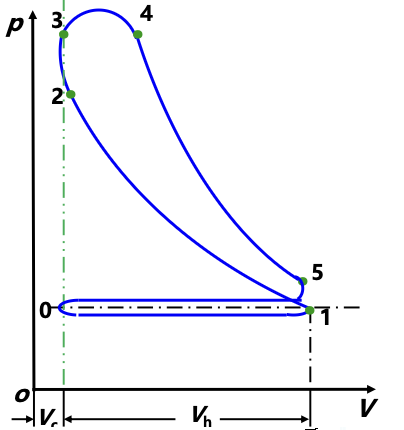
\includegraphics[width=.6\linewidth]{figures/9柴油机实际循环.png}
\end{minipage}

\noindent
\begin{minipage}
    [t]{0.35\linewidth}
    \vspace{0pt}
    \raggedright
    \pt{混合加热理想循环（萨巴德循环，柴油机）}：
    \begin{itemize}
        \item $1\to2$：等熵压缩。
        \item $2\to3$：定容吸热。
        \item $3\to4$：定压吸热。
        \item $4\to5$：等熵膨胀。
        \item $5\to1$：定容放热。
    \end{itemize}
\end{minipage}
\hfill
\begin{minipage}
    [t]{0.64\linewidth}
    \vspace{0pt}
    \centering
    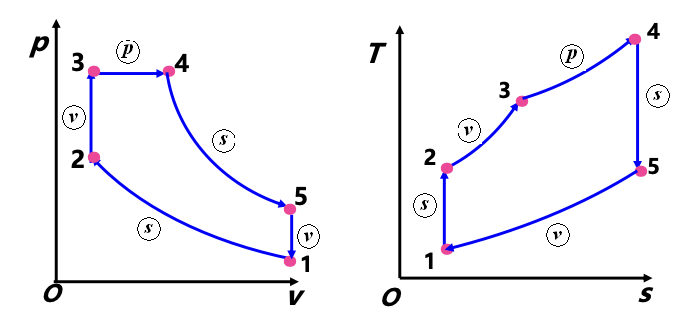
\includegraphics[width=\linewidth]{figures/9萨巴德循环.png}
\end{minipage}

\begin{itemize}
    \item \pt{循环吸热量}：$q_1=c_{\mathrm{V}}(T_3-T_2)+c_p(T_4-T_3)$，
    \item \pt{循环放热量}：$q_2=c_{\mathrm{V}}(T_5-T_1)$，
    \item \pt{热效率}：$\eta_{\mathrm{t}}=1-\frac{T_5-T_1}{(T_3-T_2)+\kappa(T_4-T_3)}$，其中 $\kappa=\frac{c_p}{c_v}$。
\end{itemize}

\pt{特性参数}

\begin{itemize}
    \item 压缩比：$\varepsilon=\frac{v_1}{v_2}$，定容增压比：$\lambda=\frac{p_3}{p_2}$，定压预胀比：$\rho=\frac{v_4}{v_3}$。
    \item \pt{等熵压缩} $1\to2$：$T_2=T_1\varepsilon^{\kappa-1}$。
    \item \pt{定容吸热} $2\to3$：$T_3=T_1\lambda\varepsilon^{\kappa-1}$。
    \item \pt{定压吸热} $3\to4$：$T_4=T_1\rho\lambda\varepsilon^{\kappa-1}$。
    \item \pt{定容放热前状态}：$T_5=T_1\lambda\rho^\kappa$。
    \item \pt{混合加热循环热效率}：$\eta_{\mathrm{t}}=1-\frac{\lambda\rho^\kappa-1}{\varepsilon^{\kappa-1}[(\lambda-1)+\kappa\lambda(\rho-1)]}$。
\end{itemize}

$\varepsilon\uparrow,\lambda\uparrow\Rightarrow\eta_{\mathrm{t}}\uparrow$；$\rho\uparrow\Rightarrow\eta_{\mathrm{t}}\downarrow$。

\divider

\noindent
\begin{minipage}
    [t]{0.35\linewidth}
    \vspace{0pt}
    \raggedright
    \pt{定压加热理想循环（狄塞尔循环，柴油机）}
    \begin{itemize}
        \item $1\to2$：等熵压缩。
        \item $2\to3$：定压吸热。
        \item $3\to4$：等熵膨胀。
        \item $4\to1$：定容放热。
    \end{itemize}
\end{minipage}
\hfill
\begin{minipage}
    [t]{0.64\linewidth}
    \vspace{0pt}
    \centering
    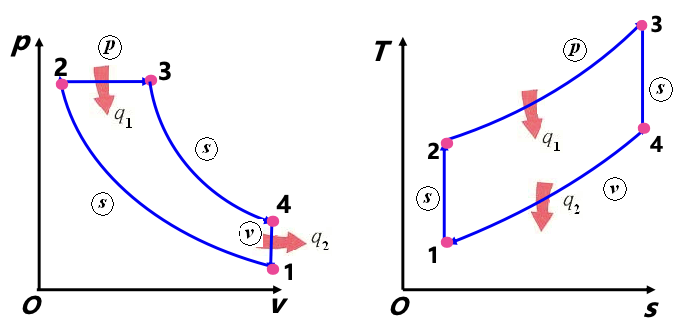
\includegraphics[width=\linewidth]{figures/9狄塞尔循环.png}
\end{minipage}

\begin{itemize}
    \item \pt{特性参数}：$\varepsilon=v_1/v_2$、$\rho=v_3/v_2$，且 $\lambda=1$。
    \item \pt{吸热量}：$q_1=c_p(T_3-T_2)$。
    \item \pt{放热量}：$q_2=c_v(T_4-T_1)$。
    \item \pt{热效率}：$\eta_{\mathrm{t}}=1-\frac{T_4-T_1}{\kappa(T_3-T_2)}$。
    \item 由混合加热循环公式令 $\lambda=1$，得 $\eta_{\mathrm{t}}=1-\frac{\rho^\kappa-1}{\kappa\varepsilon^{\kappa-1}(\rho-1)}$。
\end{itemize}

\pt{循环讨论}：
\begin{itemize}
    \item $\varepsilon$ 增大时，$\eta_{\mathrm{t}}$ 增大，$w_{\mathrm{net}}$ 增大。
    \item $\rho$ 增大时，$\eta_{\mathrm{t}}$ 降低，但 $w_{\mathrm{net}}$ 增大。
    \item 重负荷时，$\rho$ 增大、$q_1$ 增大，内部热效率下降。
    \item 温度升高会使 $\kappa$ 降低，这也是实际热效率下降的原因之一。
\end{itemize}

\divider

\pt{定容加热循环（奥托循环，汽油机）}

\begin{center}
    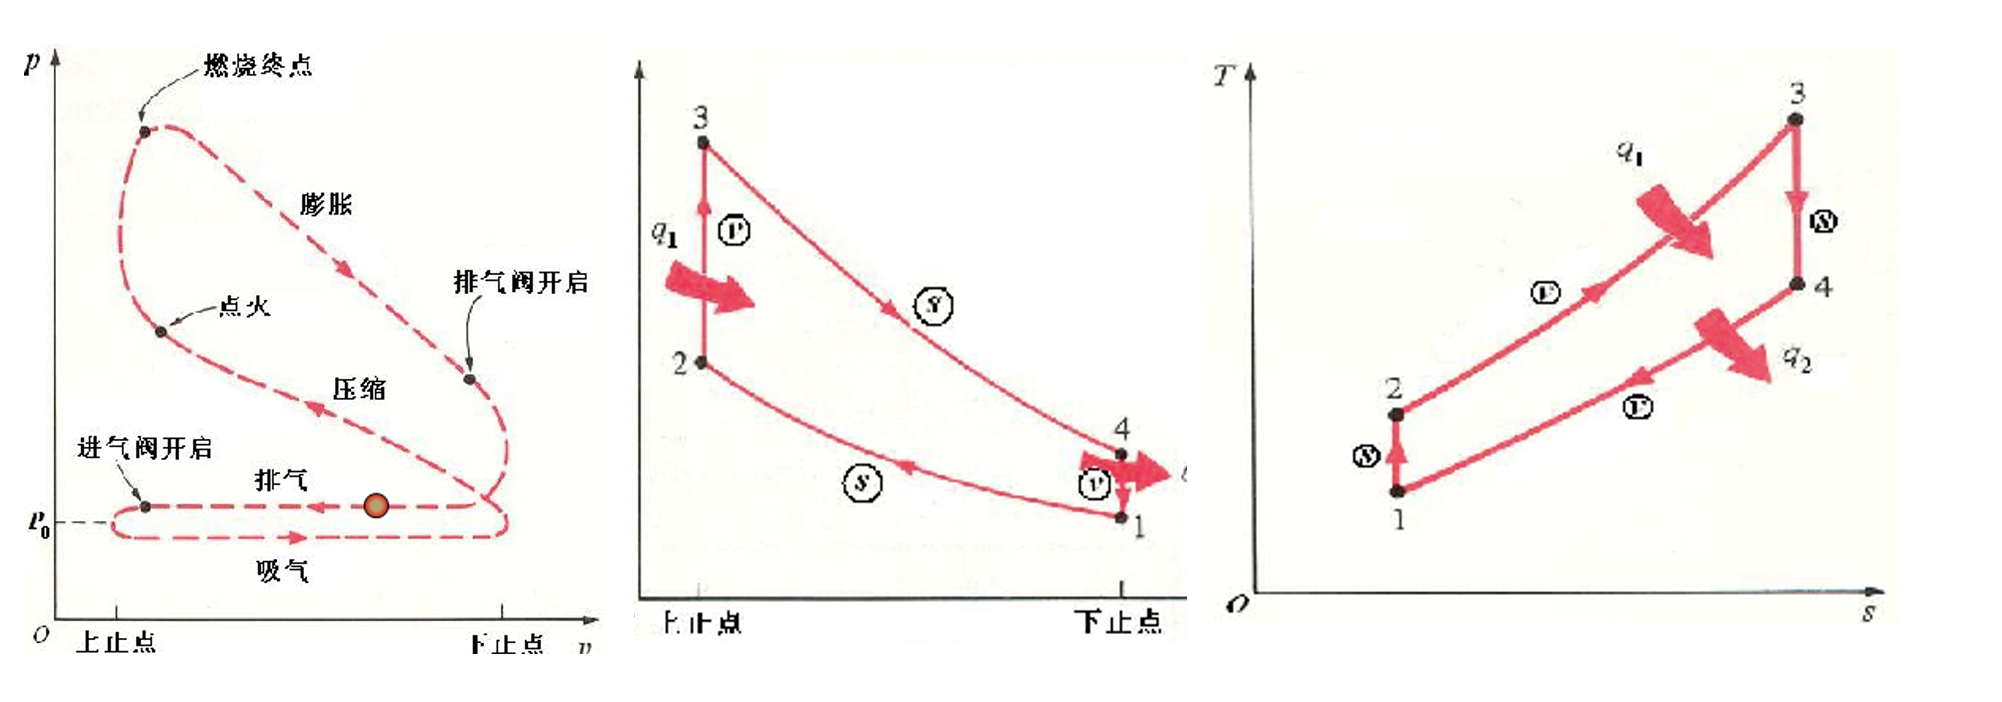
\includegraphics[width=\linewidth]{figures/9汽油机和otto循环.png}
\end{center}

\begin{itemize}
    \item $1\to2$：等熵压缩。
    \item $2\to3$：定容吸热。
    \item $3\to4$：等熵膨胀。
    \item $4\to1$：定容放热。
\end{itemize}
\par
\begin{itemize}
    \item \pt{特性参数}：$\varepsilon=v_1/v_2$、$\lambda=p_3/p_2$，且 $\rho=1$。
    \item \pt{吸热量}：$q_1=c_v(T_3-T_2)$。
    \item \pt{放热量}：$q_2=c_v(T_4-T_1)$。
    \item \pt{热效率}：$\eta_{\mathrm{t}}=1-\frac{T_4-T_1}{T_3-T_2}$。
    \item \pt{热效率}：$\eta_{\mathrm{t}}=1-\frac{1}{\varepsilon^{\kappa-1}}$。
\end{itemize}

\pt{循环讨论}：

\begin{itemize}
    \item $\varepsilon$ 增大，$\eta_{\mathrm{t}}$ 增大。
    \item $\lambda$ 增大，理想定比热条件下 $\eta_{\mathrm{t}}$ 不变，但 $w_{\mathrm{net}}$ 增大。
    \item 重负荷时，$q_1$ 增大，实际内部热效率下降，原因是温度升高导致 $\kappa$ 降低。
\end{itemize}

\divider

\pt{三种内燃机循环比较}：

\noindent
\begin{minipage}
    [t]{0.35\linewidth}
    \vspace{0pt}
    \raggedright
    \pt{压缩比相同、吸热量相同时}
    \begin{itemize}
        \item 三类循环满足 $q_{1v}=q_{1m}=q_{1p}$。
        \item 放热量关系为 $q_{2v}<q_{2m}<q_{2p}$。
        \item $\eta_{\mathrm{t}}=1-q_2/q_1$，$\eta_{\mathrm{t},v}>\eta_{\mathrm{t},m}>\eta_{\mathrm{t},p}$。
    \end{itemize}
\end{minipage}
\hfill
\begin{minipage}
    [t]{0.64\linewidth}
    \vspace{0pt}
    \centering
    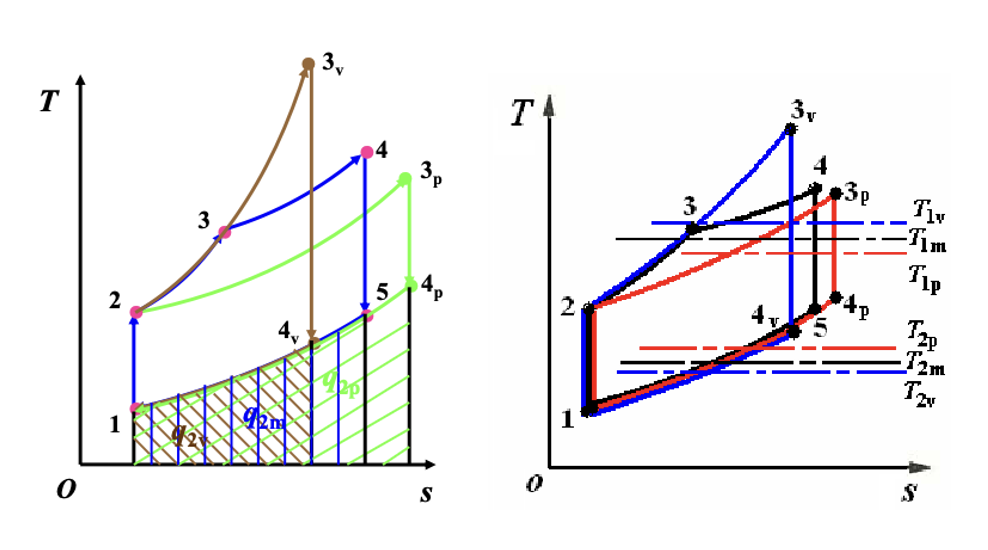
\includegraphics[width=\linewidth]{figures/9等压缩比等吸热.png}
\end{minipage}

\begin{itemize}
    \item $v$ 表示定容加热循环，$m$ 表示混合加热循环，$p$ 表示定压加热循环。
\end{itemize}

%\newcolumn

\noindent
\begin{minipage}
    [t]{0.64\linewidth}
    \vspace{0pt}
    \raggedright
    \pt{循环最高压力 $p_{\max}$ 和最高温度 $T_{\max}$ 相同时}
    \begin{itemize}
        \item $q_{2p}=q_{2m}=q_{2v}$。
        \item 吸热量关系为 $q_{1p}>q_{1m}>q_{1v}$。
        \item 因此 $\eta_{\mathrm{t},p}>\eta_{\mathrm{t},m}>\eta_{\mathrm{t},v}$。
    \end{itemize}
\end{minipage}
\hfill
\begin{minipage}
    [t]{0.35\linewidth}
    \vspace{0pt}
    \centering
    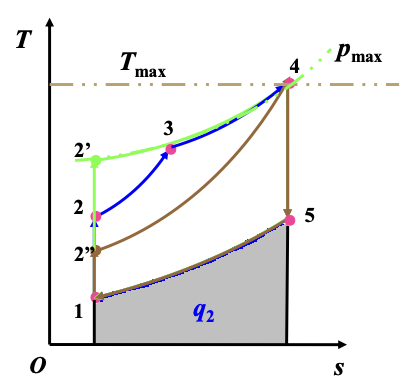
\includegraphics[width=.8\linewidth]{figures/9同最高压最高温.png}
\end{minipage}


\divider

\pt{燃气轮机装置主要构成}：压气机、燃烧室、气轮机。

\pt{燃气轮机装置特点}：实际为开式循环，工质在设备间连续流动；运转平稳，可连续输出功；启动快，到达满负荷快；压气机耗功很大，消耗气轮机产生功率的绝大部分，但装置功率重量比仍较大。

\pt{主要用途}：飞机动力、舰船动力、电站峰荷机组。

\pt{空气标准假设}：
\begin{itemize}
    \item 工质为空气，满足理想气体状态方程。
    \item 比热容取定值。
    \item 压缩和膨胀简化为等熵过程。
    \item 燃烧简化为定压吸热，排气简化为定压放热。
    \item 忽略燃油质量及燃气成分变化。
\end{itemize}

\pt{空气标准燃气轮机循环}：在上述假设下，实际开式燃气轮机循环可简化为闭式定压加热循环。

\pt{布雷顿循环（燃气轮机理想循环）}

\noindent
\begin{minipage}
    [t]{0.35\linewidth}
    \vspace{0pt}
    \raggedright
    \begin{itemize}
        \item $1\to2$：压气机内等熵压缩。
        \item $2\to3$：燃烧室内定压吸热。
        \item $3\to4$：气轮机内等熵膨胀。
        \item $4\to1$：定压放热。

    \end{itemize}
\end{minipage}
\hfill
\begin{minipage}
    [t]{0.64\linewidth}
    \vspace{0pt}
    \centering
    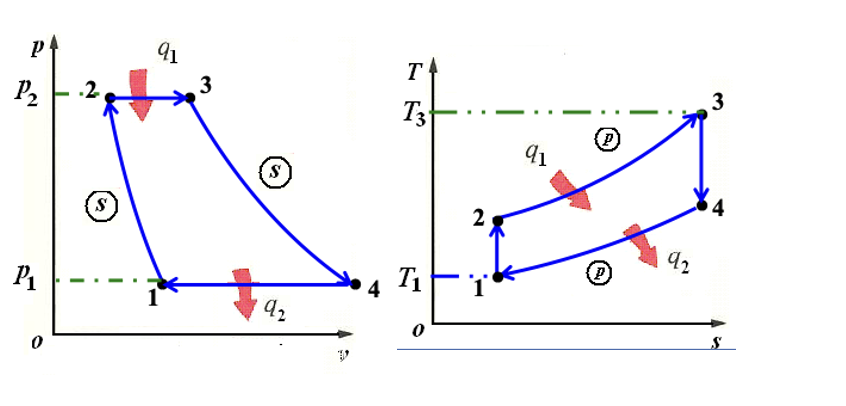
\includegraphics[width=\linewidth]{figures/9布雷顿循环.png}
\end{minipage}

\pt{循环增压比} $\pi=p_2/p_1$。\pt{循环增温比} $\tau=T_3/T_1$。

\pt{循环分析}

\begin{itemize}
    \item \pt{吸热量} $q_1=h_3-h_2=c_p(T_3-T_2)$。
    \item \pt{放热量} $q_2=h_4-h_1=c_p(T_4-T_1)$。
    \item \pt{热效率} $\eta_{\mathrm{t}}=1-\frac{q_2}{q_1}=1-\frac{T_4-T_1}{T_3-T_2}=1-\frac{T_1}{T_2}=1-\frac{1}{\pi^{(\kappa-1)/\kappa}}$。
    \item 注意：式中的 $T_1$、$T_2$ 是循环状态点温度，不是高温热源和低温热源温度。
\end{itemize}

\pt{循环分析}

\begin{itemize}
    \item $\pi$ 增大，$\eta_{\mathrm{t}}$ 增大。
    \item 理想定比热条件下，$\eta_{\mathrm{t}}$ 与循环最高温度 $T_3$ 无关。
    \item 当 $\pi$ 一定时，增大 $\tau$ 可增大吸热量和净功，但热效率不变。
    \item 循环净功为 $w_{\mathrm{net}}=c_p[(T_3-T_2)-(T_4-T_1)]$。
    \item 令 $r=\pi^{(\kappa-1)/\kappa}$，则 $w_{\mathrm{net}}=c_pT_1(r-1)(\tau/r-1)$。
    \item 当 $\tau$ 一定时，存在使 $w_{\mathrm{net}}$ 最大的最佳增压比。
    \item 最大净功条件为 $\pi=\tau^{\kappa/[2(\kappa-1)]}$。
    \item $\tau$ 升高，即 $T_3$ 升高，会使取得 $w_{\mathrm{net,max}}$ 的 $\pi$ 升高，并使 $\eta_{\mathrm{t}}$ 和 $w_{\mathrm{net,max}}$ 同时升高。
\end{itemize}

\divider

\noindent
\begin{minipage}
    [t]{0.64\linewidth}
    \vspace{0pt}
    \raggedright
    \pt{实际布雷顿循环}
    \begin{itemize}
        \item $1\to2$：不可逆绝热压缩。
        \item $2\to3$：定压吸热。
        \item $3\to4$：不可逆绝热膨胀。
        \item $4\to1$：定压放热。
    \end{itemize}
\end{minipage}
\hfill
\begin{minipage}
    [t]{0.35\linewidth}
    \vspace{0pt}
    \centering
    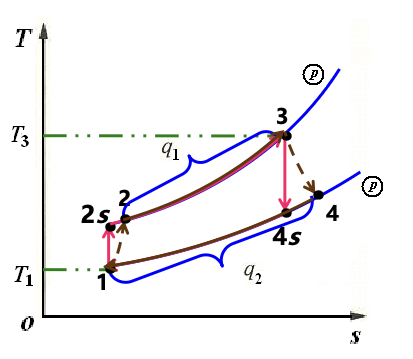
\includegraphics[width=.8\linewidth]{figures/9实际布雷顿循环.png}
\end{minipage}

\pt{压气机绝热效率}：
\begin{itemize}
    \item $\eta_{\mathrm{C,s}}=w_{\mathrm{C,s}}/w_{\mathrm{C}}'=\frac{h_{2s}-h_1}{h_2-h_1}$。
    \item 因此 $h_2=h_1+\frac{h_{2s}-h_1}{\eta_{\mathrm{C,s}}}$。
\end{itemize}
\pt{燃气轮机相对内效率}：
\begin{itemize}
    \item $\eta_{\mathrm{T}}=w_{\mathrm{t,T}}'/w_{\mathrm{t,T}}=\frac{h_3-h_4}{h_3-h_{4s}}$。
    \item 因此 $h_4=h_3-\eta_{\mathrm{T}}(h_3-h_{4s})$。
\end{itemize}
\pt{内部热效率}：
\begin{itemize}
    \item $\eta_{\mathrm{i}}=w_{\mathrm{net}}'/q_1'$。
    \item 实际净功为 $w_{\mathrm{net}}'=\eta_{\mathrm{T}}(h_3-h_{4s})-\frac{h_{2s}-h_1}{\eta_{\mathrm{C,s}}}$。
    \item 实际吸热量为 $q_1'=h_3-h_2=h_3-h_1-\frac{h_{2s}-h_1}{\eta_{\mathrm{C,s}}}$。
    \item 令 $r=\pi^{(\kappa-1)/\kappa}$，可写为 $\eta_{\mathrm{i}}=\frac{\eta_{\mathrm{T}}\tau(1-1/r)-(r-1)/\eta_{\mathrm{C,s}}}{\tau-1-(r-1)/\eta_{\mathrm{C,s}}}$。
\end{itemize}

\pt{循环讨论}

\begin{itemize}
    \item $\eta_{\mathrm{i}}$ 与 $\pi$、$\tau$ 有关。
          \subitem $\pi$ 一定时，$\tau$ 增大，$\eta_{\mathrm{i}}$ 增大。
          \subitem $\tau$ 一定时，$\pi$ 增大，$\eta_{\mathrm{i}}$ 会变化并存在极值。
    \item $\eta_{\mathrm{i}}$ 与 $\eta_{\mathrm{T}}$ 和 $\eta_{\mathrm{C,s}}$ 有关。
          \subitem $\eta_{\mathrm{T}}$ 增大、$\eta_{\mathrm{C,s}}$ 增大，会使 $\eta_{\mathrm{i}}$ 增大。
          \subitem 典型范围为 $\eta_{\mathrm{T}}=0.85\sim0.92$
          \subitem $\eta_{\mathrm{C,s}}=0.85\sim0.90$。
    \item 增大 $\tau$ 是提高燃气轮机装置性能，即提高 $w_{\mathrm{net}}$ 和 $\eta_{\mathrm{i}}$ 的重要方向。
\end{itemize}

\divider

\noindent
\begin{minipage}
    [t]{0.64\linewidth}
    \vspace{0pt}
    \raggedright
    \pt{回热}：利用燃气轮机排气预热压气机出口空气，减少燃烧室吸热。空气先被废气预热到 $T_5$，燃烧室只需要从 $T_5$ 加热到 $T_3$，吸热量为
    $q_1'=c_p(T_3-T_5)$\\
    \begin{itemize}
        \item $5$ 点：压气机出口空气在极限回热情况下能被预热到的最高状态 $T_5=T_4$
        \item $6$ 点：气轮机排气在极限回热情况下放热后能降到的最低状态 $T_6=T_2$
    \end{itemize}

\end{minipage}
\hfill
\begin{minipage}
    [t]{0.35\linewidth}
    \vspace{0pt}
    \centering
    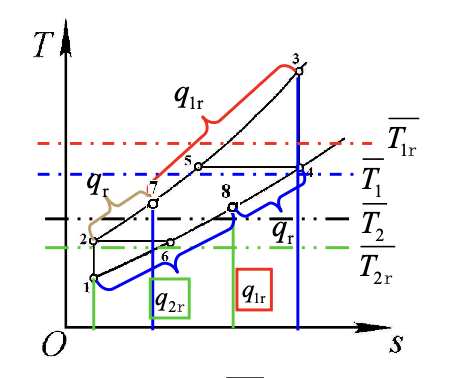
\includegraphics[width=\linewidth]{figures/9回热.png}
\end{minipage}

\begin{itemize}
    \item $7$ 点：实际回热后，压气机出口空气被预热后的状态。
    \item $8$ 点：实际回热后，气轮机排气放热后的状态。
\end{itemize}

\pt{回热度} $\sigma=\frac{\text{实际回热利用的热量}}{\text{理论极限可利用的热量}}=\frac{h_7-h_2}{h_5-h_2}=\frac{h_4-h_8}{h_4-h_6}$；

\pt{极限回热} $q_{1r}=c_p(T_3-T_5)$，$q_{2r}=c_p(T_6-T_1)$。需 $T_4>T_2$ 才有有效温差。

\noindent
\begin{minipage}
    [t]{0.7\linewidth}
    \vspace{0pt}
    \raggedright
    \pt{实际循环回热} $\sigma'=\frac{h_7-h_{2'}}{h_5-h_{2'}}$。
\end{minipage}
\hfill
\begin{minipage}
    [t]{0.29\linewidth}
    \vspace{0pt}
    \centering
    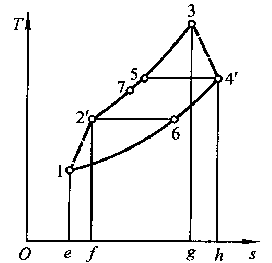
\includegraphics[width=\linewidth]{figures/9实际回热.png}
\end{minipage}

理想回热效率 $\eta_{\mathrm{t,r}}=1-\frac{q_{2r}}{q_{1r}}$，
通常 $\eta_{\mathrm{t},r}>\eta_{\mathrm{t}}$。

\divider

\pt{分级压缩中冷}：降低压气机耗功，但单独用于简单布雷顿循环时，因压气机出口温度降低、需补充更多热量，热效率不一定提高；若与回热结合，中冷增大可回热温差，可提高热效率。

\pt{分级膨胀再热}：可增加燃气轮机输出功；无回热时可能降低热效率；与回热结合时因排气温度提高、回热效果增强，可提高热效率。分级压缩中冷、分级膨胀再热和回热联合，级数趋于无穷时趋近概括性卡诺循环。

\divider

  \section{第十章\quad 蒸汽动力装置循环}

%1、2、3 ppt 全部

\pt{蒸汽动力装置}：锅炉/过热器吸热，汽轮机膨胀作功，冷凝器定压放热凝结，水泵升压送回锅炉。冷凝器不能取消：它排热并维持低背压，使循环闭合且汽轮机能充分膨胀。

\pt{水蒸气卡诺循环不采用}：温限小；膨胀末端干度 $x$ 太小，湿蒸汽冲蚀叶片；压缩两相混合物困难。实际采用朗肯循环。

\noindent
\begin{minipage}
    [t]{0.52\linewidth}
    \vspace{0pt}
    \raggedright
    \pt{朗肯循环过程}：$1$-$2$ 汽轮机绝热膨胀，$2$-$3$ 冷凝器定压放热，$3$-$4$ 水泵升压，$4$-$1$ 锅炉定压吸热（预热、汽化、过热）。
    \par\vspace{1pt}
\end{minipage}
\hfill
\begin{minipage}
    [t]{0.44\linewidth}
    \vspace{0pt}
    \centering
    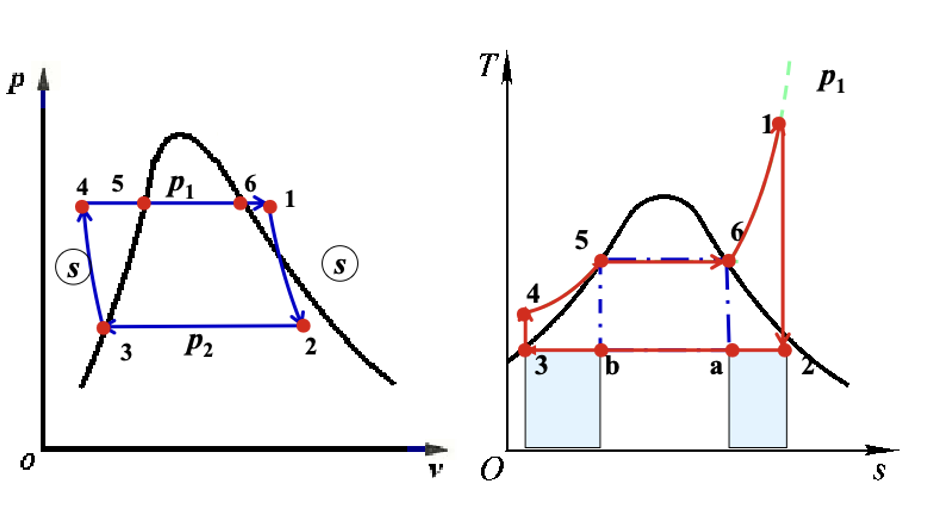
\includegraphics[width=\linewidth]{figures/10朗肯循环.png}
\end{minipage}

\pt{能量关系}：
\begin{itemize}
    \item $w_{t,T}=h_1-h_2$，$w_{t,P}=h_4-h_3$
    \item $q_1=h_1-h_4$，$q_2=h_2-h_3$
    \item $w_{\mathrm{net}}=(h_1-h_2)-(h_4-h_3)$。
\end{itemize}

\pt{朗肯循环热效率}：$\eta_{\mathrm{t}}=\frac{w_{\mathrm{net}}}{q_1}=\frac{(h_1-h_2)-(h_4-h_3)}{h_1-h_4}=1-\frac{h_2-h_3}{h_1-h_4}$。因 $w_{t,P}\ll w_{t,T}$，常取 $h_4\approx h_3$，$\eta_{\mathrm{t}}\approx\frac{h_1-h_2}{h_1-h_3}$，$w_\mathrm{net}\approx w_{t,T}$。

\pt{耗汽率}：装置每输出单位功量所消耗的蒸汽量。\pt{理想耗汽率} $d_0=\frac{1}{h_1-h_2}$；若 $h$ 用 $\mathrm{kJ/kg}$、功用 $\mathrm{kW\cdot h}$，$d_0=\frac{3600}{h_1-h_2}\,\mathrm{kg/(kW\cdot h)}$。耗汽量 $D_0=d_0P_0$。

\divider

\pt{提高初温 $T_1$}：平均吸热温度 $\bar T_1\uparrow$，$\bar T_2$ 不变，$\eta_{\mathrm{t}}\uparrow$，且末端干度 $x_2\uparrow$；受材料耐温限制。

\pt{提高初压力 $p_1$}：平均吸热温度 $\bar T_1\uparrow$，$\bar T_2$ 不变，$\eta_{\mathrm{t}}\uparrow$，但末端干度 $x_2\downarrow$，$p$ 过高，设备强度要求提高。

\pt{降低背压 $p_2$}：$\bar T_1$ 基本不变，平均放热温度 $\bar T_2\downarrow$，$\eta_{\mathrm{t}}\uparrow$，但受环境温度、冷却水温限制，不能随意降低，且 $x_2\downarrow$。

\divider

\noindent
\begin{minipage}
    [t]{0.64\linewidth}
    \vspace{0pt}
    \raggedright
    \pt{有摩阻实际朗肯循环}\\
    实际汽轮机膨胀存在摩阻和不可逆损失：
    \begin{itemize}
        \item 理想膨胀终点为 $2$，实际膨胀终点为 $2_\mathrm{act}$。
        \item 实际过程熵增大，$T-s$ 图上 $2_\mathrm{act}$ 通常位于理想等熵终点 $2$ 的右侧。
    \end{itemize}
\end{minipage}
\hfill
\begin{minipage}
    [t]{0.35\linewidth}
    \vspace{0pt}
    \centering
    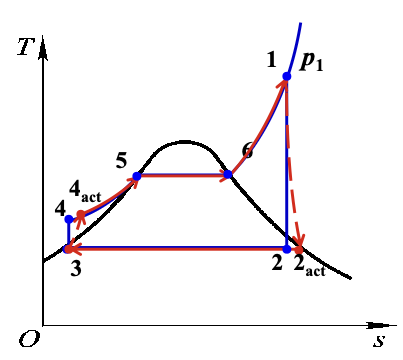
\includegraphics[width=\linewidth]{figures/10实际朗肯循环.png}
\end{minipage}

放热量增大、做功减少、效率下降。汽轮机相对内效率（汽机效率）
$\eta_T=\frac{h_1-h_{2\mathrm{act}}}{h_1-h_{2}}\approx 0.92$（近代大功率汽轮机）。

确定 $h_{2,\mathrm{act}}$ ：\pt{运行中}：测出 $p_2$ 和 $x_2$，用 $h_x=x_2h''+(1-x_2)h'$ 求湿蒸汽焓；\pt{设计中}：选定 $\eta_T$，用 $h_{2,\mathrm{act}}=h_1-\eta_T(h_1-h_2)=h_2+(1-\eta_T)(h_1-h_2)$。

$h_1-h_2$ 称为理想绝热焓降。

忽略泵功时，装置内部热效率 $\eta_i\approx\eta_T\eta_{\mathrm{t}}$；考虑机械效率 $\eta_m$ 时，有效热效率 $\eta_e=\frac{P_\mathrm{e}}{q_1}=\eta_T\eta_m\eta_{\mathrm{t}}$。实际内部耗汽率 $d_i=\frac{d_0}{\eta_T}$，耗气量 $D_i=d_iP_i$，$P_i$ 为实际内部功率。

\divider

\noindent
\begin{minipage}
    [t]{0.64\linewidth}
    \vspace{0pt}
    \raggedright
    \pt{再热循环}

    蒸汽由 $1$ 在高压汽轮机膨胀到 $b$，回锅炉再热到 $a$，再进低压汽轮机膨胀到 $2$。

    忽略泵功时，$w_{\mathrm{net}}=(h_1-h_b)+(h_a-h_2)$，$q_1=(h_1-h_3)+(h_a-h_b)$，$\eta_{\mathrm{t}}=\frac{h_1-h_b+h_a-h_2}{h_1-h_3+h_a-h_b}$。与再热压力有关
\end{minipage}
\hfill
\begin{minipage}
    [t]{0.35\linewidth}
    \vspace{0pt}
    \centering
    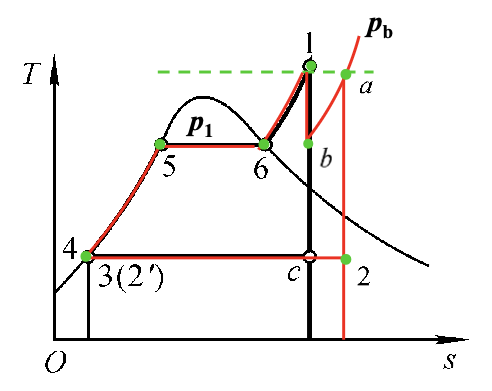
\includegraphics[width=\linewidth]{figures/10再热循环.png}
\end{minipage}

\pt{再热作用}：根本目的是提高汽轮机排汽干度；可降低耗汽率，但是会使得系统复杂
\begin{itemize}
    \item 再热压力过低时，与原循环相比，$T_{m2}$ 不变，$T_{m1}$ 下降，$\eta_\mathrm{t}$ 下降。
    \item 再热压力过高时，与原循环相比，$T_{m2}$ 不变，$T_{m1}$ 上升，$\eta_\mathrm{t}$ 上升，但 $x_2$ 改善不大。
\end{itemize}

\divider

冷凝器出来的温度过低，没有利用价值，因此不能像燃气轮机一样回热

\tdo{对不起这一块看不懂}

\pt{抽汽回热}：从汽轮机中间级抽出部分蒸汽加热给水，提高锅炉入口给水温度，减少低温段外部吸热。方式有混合式和间壁式。

\begin{center}
    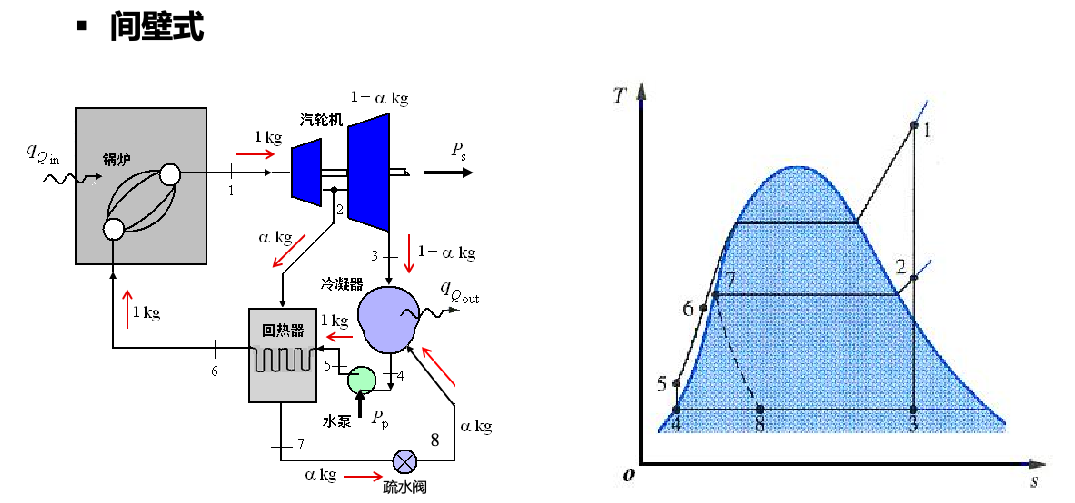
\includegraphics[width=\linewidth]{figures/10间壁式回热.png}\\
    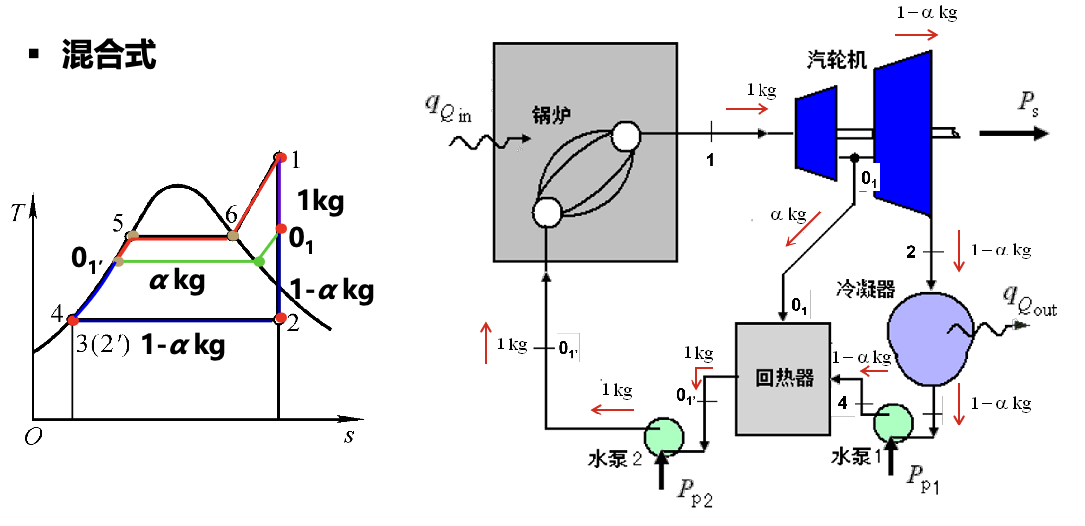
\includegraphics[width=\linewidth]{figures/10混合式回热}
\end{center}

\pt{混合式抽汽量}：主蒸汽取 $1\,\mathrm{kg}$，抽汽量 $\alpha$

抽汽量计算：
\begin{itemize}
    \item 回热器能量方程为 $(1-\alpha)h_4+\alpha h_{01}-h_{01'}=0$。
    \item 忽略泵功时，$h_4 \approx h_{2'}$。
    \item 抽汽系数为 $\alpha=\dfrac{h_{01'}-h_{2'}}{h_{01}-h_{2'}}$。
\end{itemize}

回热器不可逆损失：
\begin{itemize}
    \item 回热器熵方程写为 $(1-\alpha)s_{2'}+\alpha s_{01}-s_{01'}+S_f+S_g=\Delta s_{\mathrm{CV}}$。
    \item 稳态时取 $\Delta s_{\mathrm{CV}}=0$。
    \item 熵产为 $S_g=s_{01'}-\alpha s_{01}-(1-\alpha)s_{2'}$。
    \item 损失为 $I=T_0S_g$。
\end{itemize}

回热循环分析（忽略水泵功）：
\begin{itemize}
    \item 净功为 $w_{\mathrm{net}}=(1-\alpha)(h_1-h_2)+\alpha(h_1-h_{01})$。
    \item 也可写为 $w_{\mathrm{net}}=(h_1-h_{01})+(1-\alpha)(h_{01}-h_2)$。
    \item 吸热量为 $q_1=h_1-h_{01'}$。
    \item 放热量为 $q_2=(1-\alpha)(h_2-h_{2'})$。
    \item 热效率为 $\eta_{\mathrm{t}}=\dfrac{w_{\mathrm{net}}}{q_1}=\dfrac{(h_1-h_{01})+(1-\alpha)(h_{01}-h_2)}{h_1-h_{01'}}$。
    \item 也可写为 $\eta_{\mathrm{t}}=1-\dfrac{q_2}{q_1}=1-\dfrac{(1-\alpha)(h_2-h_{2'})}{h_1-h_{01'}}$。
\end{itemize}

回热循环与原循环比较：
\begin{itemize}
    \item 平均放热温度 $T_{m2}$ 不变；
    \item 平均吸热温度 $T_{m1}$ 上升；
    \item 因此热效率 $\eta_{\mathrm{t}}$ 提高；
    \item 回热的本质是减少低温段外部吸热，使锅炉吸热更多发生在较高温度区间。
\end{itemize}

\pt{回热循环}：$w_{\mathrm{net}}=(h_1-h_{01})+(1-\alpha)(h_{01}-h_2)$，$q_1=h_1-h_{01'}$，$q_2=(1-\alpha)(h_2-h_{2'})$。回热器熵产 $S_g=s_{01'}-\alpha s_{01}-(1-\alpha)s_{2'}$，损失 $I=T_0S_g$。

\pt{提高经济性主线}：提高平均吸热温度、降低平均放热温度、减少不可逆。再热偏向改善末级湿度，回热偏向提高平均吸热温度，大型机组常联合采用。

\divider

  \section{第十一章\quad 制冷循环}

\pt{逆向循环}：制冷循环和热泵循环均消耗外界功，把热量从低温对象转移到高温环境或供热对象。若无功输入，热量从低温传到高温会使孤立系 $\Delta S_{\mathrm{iso}}<0$，违背第二定律；实际必须满足 $\Delta S_{\mathrm{iso}}\ge 0$。

\pt{制冷系数}：$\varepsilon=\frac{q_c}{w_{\mathrm{net}}}=\frac{q_c}{q_0-q_c}$，$q_c$ 为从低温对象吸收的制冷量，$q_0$ 为向高温环境放热量。卡诺制冷循环 $\varepsilon_c=\frac{T_c}{T_0-T_c}$，温度必须用热力学温度。温差越小，理论 $\varepsilon_c$ 越大。

\pt{工程单位}：COP 即制冷装置工作性能系数；普通制冷常 $\varepsilon>1$，深冷常 $\varepsilon<1$。$1$ 冷吨约 $3.86\,\mathrm{kJ/s}$，美国制约 $3.517\,\mathrm{kJ/s}$。

\pt{热泵供热系数}：高温端供热量 $q_h=q_c+w_{\mathrm{net}}$，$\varepsilon_h=\frac{q_h}{w_{\mathrm{net}}}=\frac{q_c+w_{\mathrm{net}}}{w_{\mathrm{net}}}=1+\varepsilon>1$。热泵关注高温端放热，制冷机关注低温端吸热。

\divider

\pt{压缩空气制冷循环（逆布雷顿）}

\begin{center}
    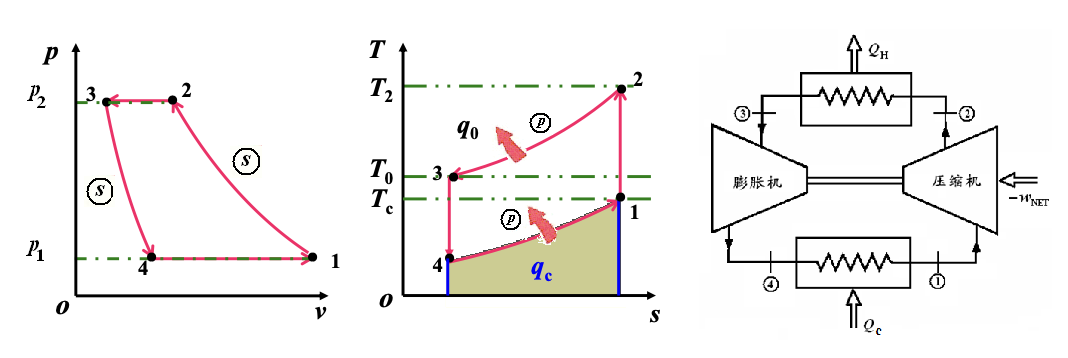
\includegraphics[width=\linewidth]{figures/11制冷循环.png}
\end{center}

$1$-$2$ 压缩机等熵压缩，$2$-$3$ 冷却器定压放热，$3$-$4$ 膨胀机等熵膨胀，$4$-$1$ 冷端定压吸热。

\pt{制冷系数}在工程上也称制冷装置的工作性能系数，即 $\mathrm{COP}$。$\varepsilon=\frac{q_\mathrm{c}}{q_0-q_\mathrm{c}}$ ，若为卡诺循环 $\varepsilon_\mathrm{c}=\frac{T_\mathrm{c}}{T_0-T_\mathrm{c}}$

深冷装置通常 $\varepsilon<1$，普通制冷装置通常 $\varepsilon>1$。

\pt{冷吨}定义：$1000\ \mathrm{kg}$、$0^\circ\mathrm{C}$ 饱和水在 $24\ \mathrm{h}$ 内冻结成 $0^\circ\mathrm{C}$ 冰所需的制冷量。$1$ 冷吨 $=3.86\ \mathrm{kJ/s}$；美国制 $1$ 冷吨 $=3.517\ \mathrm{kJ/s}$

\pt{能量关系}：制冷量 $q_c=h_1-h_4$，$q_0=h_2-h_3$，$w_{\mathrm{net}}=(h_2-h_1)-(h_3-h_4)$，$\varepsilon=\frac{h_1-h_4}{(h_2-h_1)-(h_3-h_4)}$。

\pt{理想气体定比热}情况：设 $\pi=\frac{p_2}{p_1}$，则 $T_2=T_1\pi^{(\kappa-1)/\kappa}$，$T_3=T_4\pi^{(\kappa-1)/\kappa}$，$\varepsilon=\frac{1}{\pi^{(\kappa-1)/\kappa}-1}=\frac{T_1}{T_2-T_1}$。$\pi\downarrow$ 时 $\varepsilon\uparrow$，但循环制冷量 $q_c$ 可能下降。

\newcolumn

\begin{center}
    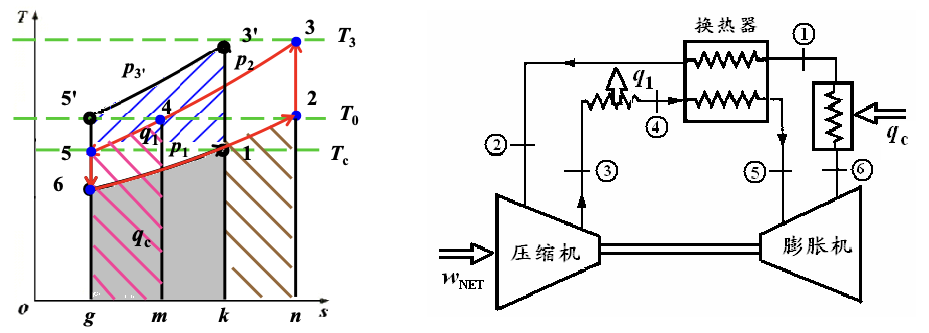
\includegraphics[width=0.8\linewidth]{figures/11回热式压缩空气制冷循环.png}
\end{center}

自冷库出来的空气（温度为 $T_1$，即低温热源温度 $T_{\mathrm{c}}$），首先进入回热器升温到高温热源的温度 $T_2$（通常为环境温度 $T_0$），接着进入叶轮式压气机进行压缩，升温、升压到 $T_3$、$p_3$，再进入冷却器，实现定压放热，降温至 $T_4$（理论上可达高温热源温度 $T_2$），随后进入回热器进一步定压降温至 $T_5$（即低温热源温度 $T_{\mathrm{c}}$），再进入叶轮式膨胀机实现定熵膨胀过程，降压、降温至 $T_6$、$p_6$，最后进入冷库实现定压吸热，升温到 $T_1$，完成循环。

\begin{itemize}
    \item 回热前：$q_1=\text{面积 }3'5'gk3'$，$q_\mathrm{c}=\text{面积 }16gk1$。
    \item 回热后：$\text{面积 }21kn2=\text{面积 }45gm4$，表示回热器内冷热流体换热量相等。
    \item 回热后：$q_\mathrm{c}=\text{面积 }16gk1$，$q_1=\text{面积 }34mn3=\text{面积 }3'5'gk3'$。
    \item 因此回热前后 $q_1$ 相等、$q_\mathrm{c}$ 相等，$w_\mathrm{net}$ 也相等，所以 $\varepsilon$ 相等。
    \item 但回热后压力比降低，课件给出 $\pi_1={p_3}/{p_2}<\pi_2={p_{3'}}/{p_1}$。
    \item 结论：回热不一定提高该理想比较下的 $\varepsilon$，但能在相同制冷量和相同净功条件下降低所需压力比，使装置更易实现。
\end{itemize}

\divider

\noindent
\begin{minipage}
    [t]{0.64\linewidth}
    \vspace{0pt}
    \raggedright
    \pt{压缩蒸气制冷循环}：
    主要设备包括压缩机、冷凝器、节流阀或毛细管、蒸发器。

    $1$-$2$ 压缩机压缩；$2$-$3$-$4$ 冷凝器放热并冷凝；$4$-$5$ 节流阀降压，近似等焓 $h_5=h_4$；$5$-$1$ 蒸发器吸热汽化。相变使单位质量制冷量大，工程制冷常用。
    \par\vspace{1pt}
    \pt{制冷系数}：$q_c=h_1-h_5=h_1-h_4$，$q_0=h_2-h_4$，$w_{\mathrm{net}}=h_2-h_1$，$\varepsilon=\frac{h_1-h_4}{h_2-h_1}$。不能用 $\frac{T_1-T_4}{T_2-T_1}$ 代替焓差。
\end{minipage}
\hfill
\begin{minipage}
    [t]{0.35\linewidth}
    \vspace{0pt}
    \centering
    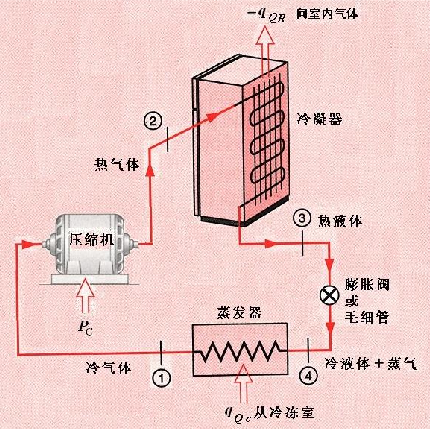
\includegraphics[width=\linewidth]{figures/11压缩制冷设备.png}
\end{minipage}

\divider

\noindent
\begin{minipage}
    [t]{0.35\linewidth}
    \vspace{0pt}
    \raggedright
    \pt{$\log p$-$h$ 图}：横坐标为焓 $h$，纵坐标为 $\log p$，适合压缩蒸气制冷循环查图计算。核心用途是确定各状态点后，直接用焓差求制冷量、压缩功、放热量和制冷系数。

    \begin{itemize}
        \item 定压过程在 $\log p$-$h$ 图上近似为水平线。
        \item 蒸发器过程 $5$-$1$ 位于低压线，即蒸发器压力线上。
        \item 冷凝器过程 $2$-$4$ 位于高压线，即冷凝器压力线上。
        \item 节流过程 $4$-$5$ 近似等焓，故 $h_5=h_4$，在图上近似为竖直线。
    \end{itemize}


\end{minipage}
\hfill
\begin{minipage}
    [t]{0.64\linewidth}
    \vspace{0pt}
    \centering
    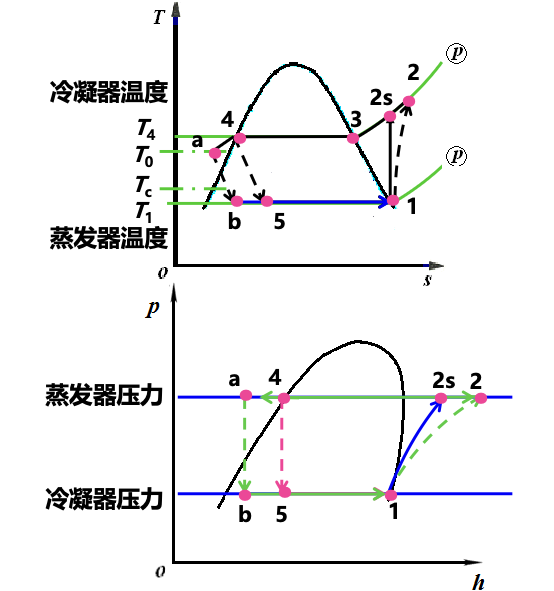
\includegraphics[width=\linewidth]{figures/11logpht.png}
\end{minipage}

\begin{itemize}
    \item 压缩过程 $1$-$2s$ 表示理想等熵压缩，$1$-$2$ 表示实际压缩。
\end{itemize}

\pt{循环计算}：
\begin{itemize}
    \item 制冷量：$q_c=h_1-h_5=h_1-h_4$。
    \item 冷凝器放热量：$q_1=h_2-h_4$。
    \item 压缩机耗功：$w_{\mathrm{net}}=h_2-h_1$。
    \item 制冷系数：$\varepsilon=\frac{q_c}{w_{\mathrm{net}}}=\frac{h_1-h_4}{h_2-h_1}$。
    \item 过冷循环：$\varepsilon_{\mathrm{SC}}=\frac{h_1-h_b}{h_2-h_1}$。
\end{itemize}

\pt{液体过冷}：冷凝器出口由 $4$ 过冷到 $b$，节流后焓降低，$\varepsilon_{\mathrm{SC}}=\frac{h_1-h_b}{h_2-h_1}>\varepsilon$，单位质量制冷量增大。

\pt{提高压缩蒸气制冷系数}：降低冷凝温度、提高蒸发温度、减少不可逆压缩损失、采用液体过冷、减少节流损失。

\pt{制冷剂要求}：
\begin{itemize}
    \item \pt{热力性质}：对应制冷装置工作温度时，饱和压力应适中；汽化潜热应大，这样单位质量制冷量 $q_\mathrm{c}$ 较大；临界温度应高于环境温度，便于在环境温度附近冷凝；蒸气比体积应小，有利于减小压缩机体积流量和设备尺寸；导热系数应大，有利于换热器传热；蒸发压力不宜低于环境压力，避免系统在负压下运行并吸入空气；三相点应低于制冷循环下限温度，避免工作范围内出现固化问题；在 $T$-$s$ 图上，上、下界限线应较陡峭，使冷凝更接近定温放热，并减少节流引起的制冷能力损失。
    \item \pt{其他性质}：对环境友善；安全无毒；溶油性好；化学稳定性好。
\end{itemize}

\noindent
\begin{minipage}
    [t]{0.35\linewidth}
    \vspace{0pt}
    \raggedright
    \pt{热泵循环}：热泵循环与制冷循环使用相似的逆向循环装置

    \pt{供热系数}：$\varepsilon'=\frac{w_{\mathrm{net}}+q_2}{w_{\mathrm{net}}}=1+\frac{q_2}{w_{\mathrm{net}}}>1$
\end{minipage}
\hfill
\begin{minipage}
    [t]{0.64\linewidth}
    \vspace{0pt}
    \centering
    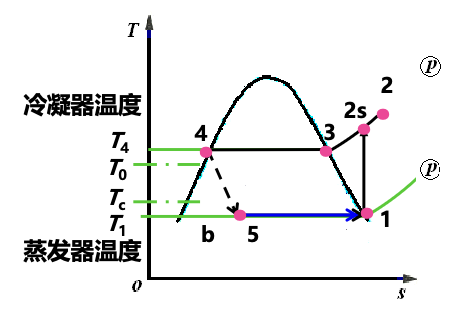
\includegraphics[width=\linewidth]{figures/11热泵循环.png}
\end{minipage}

\pt{供暖例子}：
\begin{itemize}
    \item 工业锅炉效率为 $\eta_{\mathrm{B}}=0.7$，则 $Q=Q_{\mathrm{a}}\eta_{\mathrm{B}}=0.7Q_{\mathrm{a}}$。
    \item 电厂热效率为 $\eta_{\mathrm{t}}=0.35$，热泵供暖系数为 $\varepsilon'=3$。
    \item 若用一次能源 $Q_{\mathrm{a}}$ 发电后驱动热泵，则供热量为 $Q=Q_{\mathrm{a}}\eta_{\mathrm{t}}\varepsilon'=1.05Q_{\mathrm{a}}$。
    \item 这个例子说明，在给定参数下，热泵供暖可比直接锅炉供暖获得更高的有效供热量。
\end{itemize}

\begin{center}
    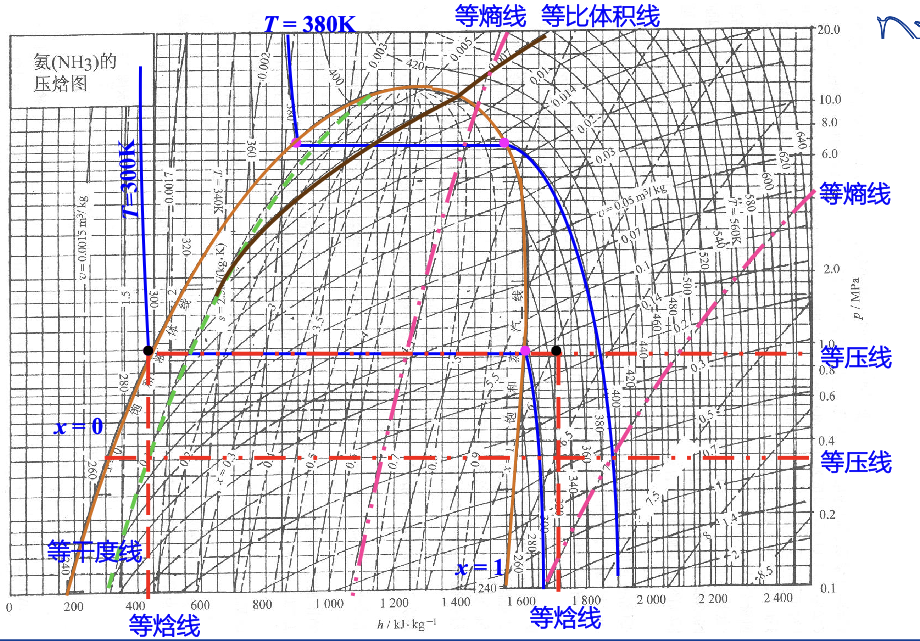
\includegraphics[width=\linewidth]{figures/11氨焓压图.png}
\end{center}

孩子们这是啥
\divider

  %\section{后文}

感谢水源用户 \href{https://shuiyuan.sjtu.edu.cn/u/milvoid/summary}{@Milvoid} 的 \href{https://shuiyuan.sjtu.edu.cn/t/topic/471743}{CheatingSheetTemplate} 模版，github 地址 \url{https://github.com/Milvoid/CheatingSheetTemplate}

感谢 chatgpt、gemini、codex 老师的大力协助

感谢群 U 们的 issue

特别感谢

\begin{itemize}
    \item 初音未来
    \item Queen
    \item 轻音少女
    \item 飞八分钱 Phonk
    \item 哈基米音乐
    \item 理堂金曲
    \item 念张师
\end{itemize}

等提供的精神支持
\end{cheatsheet}
\end{document}
